\documentclass[12pt,
paper=a4,				
DIV=calc,		  % führt die Satzspiegelberechnung neu aus
%oneside,		  % einseitiger Druck
BCOR=16mm,	  % Bindekorrektur
headinclude,
%footinclude,
openany
]{scrbook}


%****************
% define medatata
%________________
\def\Title{An Example Document}
\def\Author{Some Name}
\def\Subject{An Example Document}
\def\Keywords{LaTeX,Example,Document}
 
%***************************************************************************
% \convertDate converts D:20080419103507+02'00' to 2008-04-19T10:35:07+02:00
%___________________________________________________________________________
\def\convertDate{%
    \getYear
}
 
{\catcode`\D=12
 \gdef\getYear D:#1#2#3#4{\edef\xYear{#1#2#3#4}\getMonth}
}
\def\getMonth#1#2{\edef\xMonth{#1#2}\getDay}
\def\getDay#1#2{\edef\xDay{#1#2}\getHour}
\def\getHour#1#2{\edef\xHour{#1#2}\getMin}
\def\getMin#1#2{\edef\xMin{#1#2}\getSec}
\def\getSec#1#2{\edef\xSec{#1#2}\getTZh}
\def\getTZh +#1#2{\edef\xTZh{#1#2}\getTZm}
\def\getTZm '#1#2'{%
    \edef\xTZm{#1#2}%
    \edef\convDate{\xYear-\xMonth-\xDay T\xHour:\xMin:\xSec+\xTZh:\xTZm}%
}
 
\expandafter\convertDate\pdfcreationdate 
 
%**************************
% get pdftex version string
%__________________________
\newcount\countA
\countA=\pdftexversion
\advance \countA by -100
\def\pdftexVersionStr{pdfTeX-1.\the\countA.\pdftexrevision}
 
 
%*********
% XMP data
%_________
\usepackage{xmpincl}
%\includexmp{pdfa-1b}
 
%********
% pdfInfo
%________
\pdfinfo{%
    /Title    (\Title)
    /Author   (\Author)
    /Subject  (\Subject)
    /Keywords (\Keywords)
    /ModDate  (\pdfcreationdate)
    /Trapped  /False
}
 

\hyphenation{nano-wires nano-wire nano-structures nano-struc-tured TRI-DYN COS-IPO}
\usepackage[utf8]{inputenc}
\usepackage{color}
\usepackage{graphicx}
\setcapindent{1em}
\setkomafont{caption}{\small}
%\usepackage{wrapfig}
\usepackage{sidecap}
\usepackage{amsmath}
\usepackage{nicefrac}


\bibliographystyle{alpha} 
\newcommand{\fett}[1]{{\bf #1}}
\newcommand{\TODO}[1]{{\LARGE{\textcolor{red}{\emph {#1 }}}}}
\clubpenalty10000
\widowpenalty10000

\usepackage{setspace}
%\singlespacing
\onehalfspacing
%\doublespacing
%\setstretch{1.1}


\makeindex
\begin{document}



\titlehead{Friedrich Schiller Universität Jena\\
PAF}
\subject{Dissertation}
\title{High-Fluence Ion Beam Irradiation of Semiconductor Nanowires}
\author{Andreas Johannes}
\date{July 2015}
\maketitle







\tableofcontents

\chapter{Introduction}
\pagenumbering{arabic}
\setcounter{page}{1}
%\let\clearpage\relax


%


%We are living in an era dominated by the information technology. There is virtually no part of life not influenced by the continuing advances in the digital world and semiconductors, especially silicon, are at the base of each and every logic unit dealing in `ones' and `zeros'. Silicon therefore quickly became one of the most studied materials, catching up with the previously dominating iron and its various alloys with other elements, steel.

Technological progress generally shows a competition between the optimization of the dominating technology and the development of fundamentally new operation principles. An example of this competition is recorded in the ``International Technology Roadmap for Semiconductors'', which aims to guide the scaling of digital devices to follow ``Moore's Law'' of improved performance, and the white paper ``Towards a `More-than-Moor' roadmap'', which examines opportunities to include non-digital functionality where performance does not necessarily have to scale with size. Both are available at the ITRS website  \cite{map_http://www.itrs.net/_2015}. A shift in operating principle is found, for example, in data storage, which changed fundamentally when the effect of giant magneto-resistance (GMR) was discovered in 1988. 
This quickly formed the basis for the standard hard-drives (HDD) and HDDs soon dominated PC data storage. Nowadays, the much older principle of flash memory is making a come-back in solid state drives (SSD), which begin to replace HDDs. They owe their viability (cost, speed and storage density) almost entirely to the advanced miniaturization, allowing the production of a floating gate for a transistor on a scale down to tens of nanometers per single $bit$, while producing \emph{billions} of $\nicefrac{bits}{cm^{2}}$. This shows, that it is not \emph{a priori} possible to discern with certainty which approach is going to produce the best results, so that much room is left for open minded fundamental research in general and on semiconductors in particular.

In the wake of the miniaturization used for the improvement of IT hardware technology, the new, multi-disciplinary field of nanotechnology has emerged. The scope of the field is illustrated by the high number of journals dedicated to research at the nanoscale. This includes semiconductor science, but in the leading journals \emph{ACS Nano} \cite{acs_nano_http://pubs.acs.org/journal/ancac3_2015}, \emph{Advanced Materials} \cite{advanced_materials_http://www.advmat./_2015}, \emph{Advanced Functional Materials} \cite{advanced_functional_materials_http://onlinelibrary.wiley.com/journal/10.1002/issn1616-3028_2015}, \emph{Nano Letters} \cite{nano_letters_http://pubs.acs.org/journal/nalefd_2015}, \emph{Nature Nanotechnology} \cite{nature_nanotechnology_http://www.nature.com/nnano_2015}, \emph{Nano Today} \cite{nano_today_http://journals.elsevier.com/17480132/nano-today/_2015}, \emph{Nanotoxicology} \cite{nanotoxicology_http://www.informahealthcare.com/nan_2015}, \emph{Small} \cite{small_http://www.small-journal.com/_2015} and others, fundamental research and applications of nanoscale devices and effects from all natural sciences are published.

The specific class of nanomaterials investigated in this thesis are semiconductor nanowires, which have gained a significant amount of  interest \cite{huang_room-temperature_2001,cui_nanowire_2001,duan_indium_2001,xia_one-dimensional_2003,lieber_functional_2007}. `Nanowire' is a term used for many morphologies, but it seems a reasonable name for structures with a cross-section that is between $1 \times 1$ and $1000 \times 1000\,nm^2$ and a large length to form a high aspect ratio. One of the general aspects of this shape and also of nanostructured materials in general, is that the surface properties play a dominating role. This is simply caused by the fact, that there is a lot of surface per volume of material. As the surface to volume ratio in general is proportional to $1/r$ for a body with a characteristic constraining length of $r$, it gets very large for small structure sizes.

The wire shape has an inherent advantage over three dimensionally constrained particles (nanoclusters, quantum dots etc.), in that it is easier to define contacts and drive a current through a nanoscale wire than through a nanoscale dot. Incidentally, the idea to combine this specific advantage of nanowires with new properties obtained by the stronger three dimensional confinement of quantum dots is the main idea behind the `Deutsche Forschungsgemeinschaft' (DFG) project ``wiring quantum dots", which funded this work. 

The defining property of semiconductors is the ability to dramatically change their electronic properties by adding impurities \cite{sze_physics_2006}. As ion beam irradiation can be used to `mix' (i.e. dope) virtually any target material with a precisely controlled number of atoms of practically any element, it was and is a key part in the processing and development of semiconductor technologies. 

In general, ion beam doping has the advantage over doping during the synthesis of nanostructures, since it is not inherently limited by the chemical potentials and thermodynamics which typically have to be carefully controlled for the synthesis of nanostructures. It is a non-equilibrium physical process by which different elements can forcefully be introduced into a target matrix with much higher energies than those involved in chemical bonding. The extent of disorder created in the target during this bombardment, whether the intermixing is thermodynamically stable and whether a desired (crystalline) order can be reestablished by thermal annealing is in the focus of ion-beam physics. A good background on this can be gained from dedicated literature \cite{ziegler_stopping_1985,eckstein_computer_1991,nastasi/mayer/hirvonen_ion-solid_2008,schmidt_ion_2012}.

%Scaling down material to the nanoscale becomes interesting when the structure size reaches the characteristic dimension of the effect governing the physical properties of interest. Then new, mesoscopic and quantum mechanical properties can emerge. As an example, the changed light-matter interaction in structures of the dimension of the wavelength of light is investigated in the field of nano-photonics and plasmonics \cite{saleh_fundamentals_2007,maier_plasmonics:_2007}.


Typical ion ranges for the doping of semiconductors lie in the range of $10$-$100\,nm$. Therefore, ion beam irradiation of nanostructures of the same dimension will show some interplay between the irradiated structures' dimensions and the ion range. The many practical applications of the combination of ion beams and nanostructures warrants general investigations of the nanostructure - ion beam interaction and the topic has therefore gained increased interest very recently \cite{borschel_ion-solid_2012,greaves_enhanced_2013,nietiadi_sputtering_2014,johannes_ion_2015,urbassek_sputter_2015}.  

A specific example in which the combination of nanostructures and ion beams is advantageous is the ion irradiation of diamond to create nitrogen-vacancy clusters. The diamond is nanostructured to facilitate efficient extraction of light, while ion irradiation with nitrogen creates nitrogen-vacancy clusters very effectively. These are interesting as promising components in a future quantum information device \cite{babinec_diamond_2010}. The precise control ion irradiation gives, makes it possible to implant a well defined number of ions with reasonable spacial accuracy. This control is extravagantly demonstrated by the possibility of single ion irradiation, shown in references \cite{meijer_concept_2006,ohdomari_single-ion_2008}. 

In addition to this extremely low ion fluence example of ion irradiation, the next two examples of the concurrence of nanotechnology and ion-irradiation led more or less directly into the investigations into high fluence irradiation presented in this dissertation. Firstly there is the search for a diluted magnetic semiconductor for which $Mn$ doped $GaAs$-nanowires are a good candidate. As $GaAs$ nanowires typically grow above $450^\circ C$ but $MnAs$ segregates from $Ga_{(1-x)}Mn_xAs$ at around $350^\circ C$ \cite{dietl_engineering_2006,sadowski_gaasmnas_2011}, there is no straightforward way to dope $GaAs$-nanowires with high concentrations of $Mn$ during their growth. However, it can be achieved by implanting $Mn$ in $GaAs$-nanowires. Best results are achieved when the irradiation is performed at elevated temperatures, hot enough to minimize disorder introduced by the ion beam, but cold enough to prevent segregation of $MnAs$ \cite{borschel_new_2011,paschoal_hopping_2012,borschel_ion-solid_2012,kumar_magnetic_2013,paschoal_magnetoresistance_2014}. 

Conversely, the ``wiring quantum dots'' project aimed to utilize the segregation of ion-implanted material in a nanowire to form nanowires decorated with nanoclusters. When $Si$ nanowires are irradiated with high fluences of $In^+$ and $As^+$ and subsequently annealed with a flash-lamp, separated $InAs$ slices form within the $Si$ nanowires \cite{prucnal_iii-v_2014,glaser_personal_2015}. The supersaturation of $Si$ with $In$ and $As$ by ion implantation can thus be utilized to create $Si$-$InAs$ nanowire hetero-structures from a $Si$ nanowire template in a relatively straightforward manner.
 
A further important example of the intersection of nanotechnology and ion beams is found in the ubiquitous focused ion beam (FIB) systems. The production and development of many of the novel nanoscale devices on the horizon often requires the precise ion beam milling that FIBs provide with a resolution of few nanometers \cite{kranz_integrating_2001,george_nanopore_2010,chalapat_self-organized_2013}. In all the examples given so far, and virtually per definition in the last one, the typical structure sizes irradiated are in the same order of magnitude at the range of the impinging ions. Understanding how this affects the ion-matter interaction can be crucial to the successful outcome of the respective experiments.

In the effort to understand principles and fundamental interactions on the nanometer length scales, nanowires are a very good model system to investigate, as their geometry is fully characterized by their height and radius. Spheres, which would have a degree of freedom less, are more difficult to handle, as the unavoidable proximity of a substrate may influence their behavior \cite{hu_burrowing_2002,klimmer_size-dependent_2009,moller_tri3dyn_2014,johannes_ion_2015}. The understanding of the ion-nanostructure interaction gained by investigating irradiated nanowires is principally transferable to any nanostructure. However, this can hardly be done in any general way explicitly, as the possible shapes of nanostructures are uncountable. This dissertation adds to the growing field of nanostructure - ion beam interaction the discussion of three effects which are especially important in high fluence irradiation and dedicates a separate chapter to each. 
 
\begin{description}
  \item[\normalfont Chapter 3 - Sputtering of Nanowires] \hfill \\
  In the dissertation of Dr. C. Borschel \cite{borschel_ion-solid_2012} the program \emph{iradina} \cite{borschel_ion_2011} was developed and used to simulate the ion irradiation of nanostructures. It predicts an enhanced, diameter-dependent sputter yield in nanostructures. This chapter discusses the simulation and compares its predictions with experimentally obtained diameter-dependent sputtering in nanowires. Some first results on the sputtering during $Mn$ irradiation of $GaAs$-nanowires are published elsewhere \cite{johannes_enhanced_2014}. The results presented here are on $Ar$ irradiated $Si$-nanowires. They were obtained in close cooperation with Stefan Noack \cite{noack_sputter_2014} in his M.Sc. and also published in reference \cite{johannes_anomalous_2015}.
  \item[\normalfont Chapter 4 - High Doping Concentrations in Nanowires] \hfill \\
  The concentration of dopants does not follow a linear increase with the fluence of ions implanted for high fluences. It has already been observed that sputtering of the target will dynamically change its composition during the ion irradiation in addition to the intended change by incorporation of the ions within the target material \cite{moller_tridyn_1984,moller_tridyn-binary_1988,miyagawa_computer_1991,sigmund_alloy_1993,eckstein_oscillations_2000}. This effect is enhanced in nanostructures, first, since the sputtering is enhanced when compared to bulk samples as shown in the preceding chapter, but also since there is simply less material. Hence, the effect of removing material by sputtering already becomes significant at lower fluencies in nanostructures than in bulk. The presented results are acquired by compositional analysis using nano-XRF performed on 175\,keV Mn$^+$ ion irradiated ZnO nanowires \cite{johannes_enhanced_2014}. They are discussed in comparison to a pseudo-dynamic simulation performed using results from \emph{iradina}.
  \item[\normalfont Chapter 5 - Plastic Flow in Silicon Nanowires] \hfill \\
  In the high ion fluence irradiated $Si$ nanowires an unexpected tendency of the nanowires to become shorter was observed. This chapter presents a dedicated investigation into this plastic deformation of $Si$ under ion irradiation which has been previously seen only in high energy ($\ge\,MeV$) ion irradiations \cite{volkert_stress_1991,trinkaus_viscoelastic_1995,hedler_amorphous_2004,hedler_boundary_2005}.
\end{description}



%\chapter{Background}

This chapter will provide a general scientific context for this dissertation. First a general outline of energetic ion-solid interaction is given. Then the possibilities of simulating this ion-solid interaction are discussed with an emphasis on those effects that will be relevant to the experiment in this thesis. 

\section{Ion-solid interaction}

\subsubsection{Energy loss}

An energetic ion impinging on a solid will lose its kinetic energy to the solid in a variety of processes. The stopping power $S$ is well described for a large energy range by the Bethe (sometimes ``Bethe-Bloch'') formula derived using the Born approximation perturbation theory on the impact between the `fast' ion and the `slow' electrons in the solid: 

\begin{equation}
S = \frac{dE}{dx} = - A \cdot \frac{\rho\,Z_2\cdot Z_1^2}{\beta^2} \cdot \left[ln\Big(\frac{B\cdot\beta^2}{Z_2\cdot(1-\beta^2)}\Big)-\beta^2\right] ,
\end{equation}


with $A$ and $B$ positive combinations of constants, $\rho$ the density and $Z_2$ the atomic number of the target, $Z_1$ and $\beta = v/c$ the atomic number and relativistic velocity of the ion. Corrections to this formula are especially necessary for low ion energies, but in detail they are dependent on the target composition, the ion energy and ion mass in a non-trivial way. Figure \ref{stopping} and the following discussion illustrates stopping regimes and why corrections are required to the Bethe formula. It is adapted from \cite{sigmund_stopping_2004}.

\begin{figure}
	\centering
		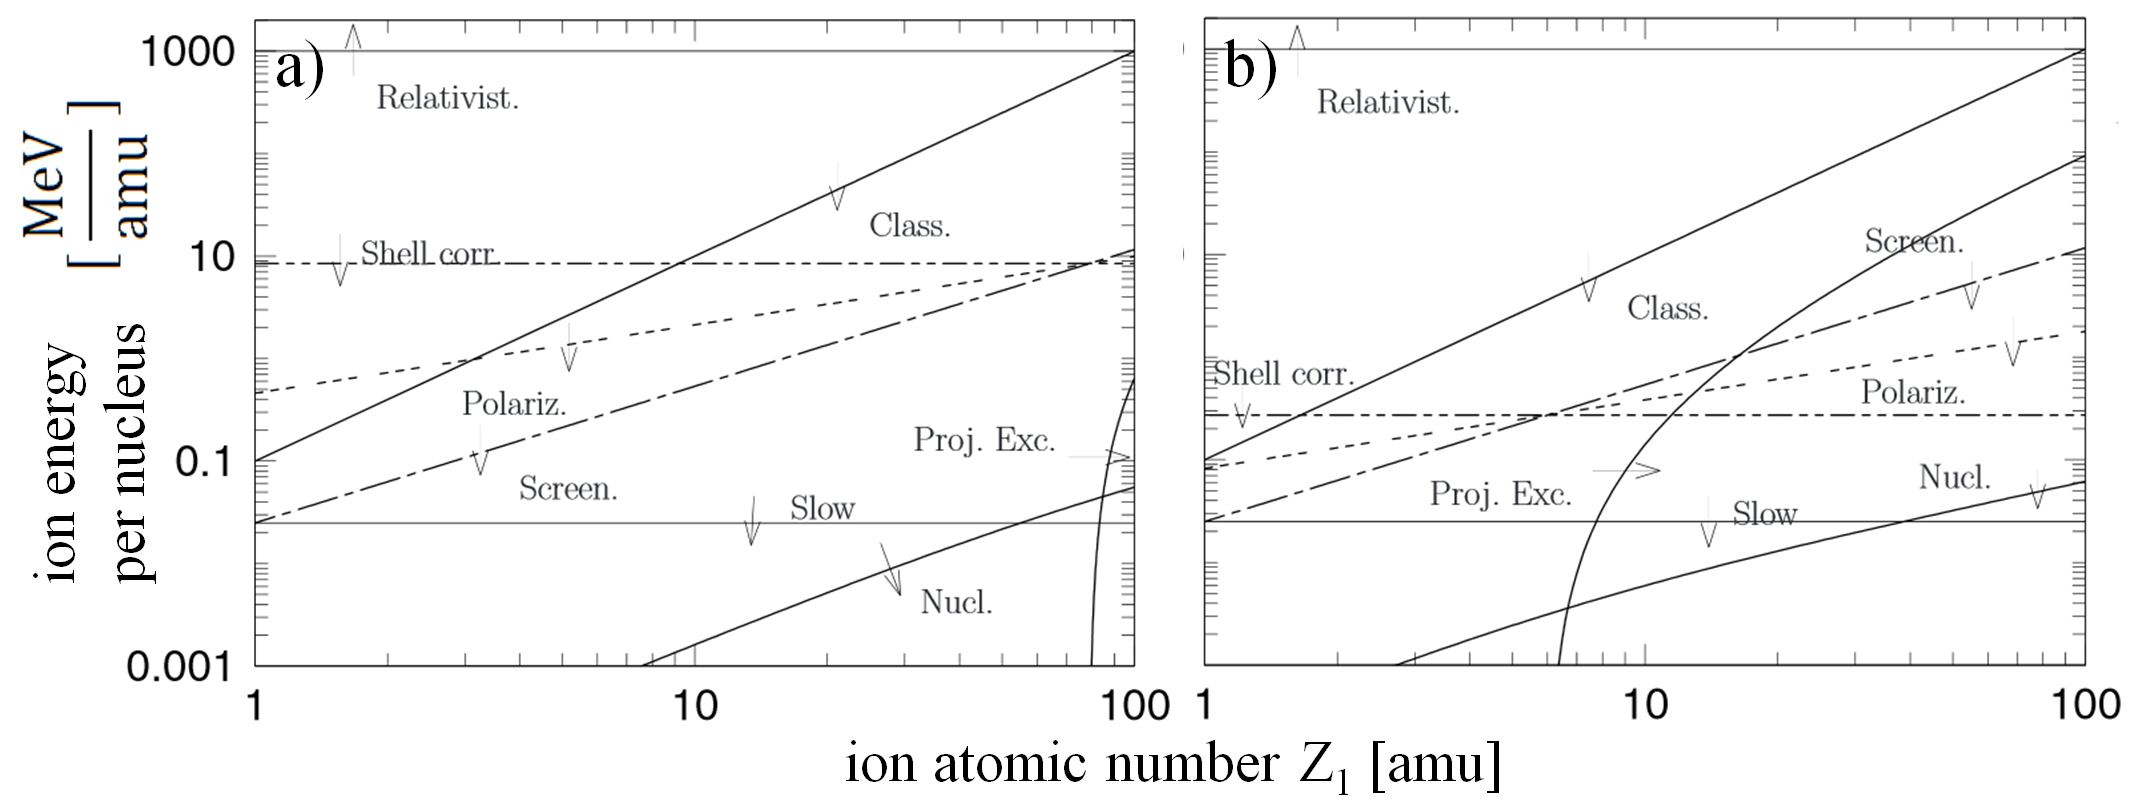
\includegraphics[width=.95\textwidth]{images/StoppinginAuandC.png}
	\caption{Illustration of the dominant effects on the stopping power for an ion of mass $Z_1$ and energy $E$ in $Au$ a) and $C$ b). Adapted from \cite{sigmund_stopping_2004}.} 
	\label{stopping}
\end{figure} 

At high ion energies ($ > 1\,GeV/amu$, labeled ``Relativist.'') highly relativistic effects have to be taken into account. At these energies we have, for example, Cherenkov radiation. Typically, nuclear reactions and resonances also occur at high ion energies. They may play a role at lower energies, especially for light ion-target combinations. However, as nuclear reactions may change the ion species, their cross sections are usually treated separately from the stopping power.

The horizontal line labeled ``Shell corr.'' marks the Thomas-Fermi velocity ($Z_2^{2/3}v_0$) of the target electrons. The constant $v_0 = e^2/\hbar = 25\,keV/amu$ is the Bohr velocity. In the parameter-space below this line the ion is moving at speeds comparable to that of the electrons in the target. In the low energy area below the line labeled ``Slow'' ($25\,keV/amu$) the ion is traveling at speeds below the Bohr velocity of the target electrons. Here the ion velocity is only comparable to that of the valence electrons in the solid. Both these points mean that the actual electron density distribution and chemical nature of the solid becomes relevant, which is of course not considered in the general Bethe formula. This makes a general and accurate theoretical prediction of electronic stopping impossible for low ion energies. Specific ion-target combinations require specific investigations.

Above the line showing the Thomas-Fermi velocity of the ion ($v = Z_1^{2/3}v_0$, ``Screen.'') the ion can be assumed to be stripped of all its electrons. Below, a screening function must consider the effective charge of the ion. Below the curve labeled ``Proj. Ext.'' the ion (projectile) carries a comparable number of electrons to the target making excitation processes in the electronic configuration of the ion significant.

For ion velocities $v < (Z_1Z_2)^{1/3}v_0$ (labeled ``Polariz.'') a higher order ($Z_1^3$) correction term to the Bethe formula becomes relevant due to the Barkas-Andersen effect. Below the line marked ``Class.'' ($Z_1^2\cdot 100\,keV/amu$) classical Bohr orbits can be used for electrons around the ion, this is a \emph{sufficient} criterion for the derivation of the Bethe formula not a \emph{necessary} one.

Finally, not be confused with the nuclear reactions already mentioned, in the region marked ``Nucl.'', at low ion energies and for large ions, the interaction with the electronic system becomes weak. Here the contribution of the coulomb interaction between ion and individual target atoms as a whole become the main contribution to slowing the ion. This is called nuclear stopping in contrast to the electronic stopping discussed so far, as kinetic energy is transferred to the target nuclei, not just the electrons.

Those ion-solid interaction processes which are specific to the properties of the target material can be used to characterize the material. These methods are summarized as ion beam analysis (IBA). A confident and comprehensive review of the possibilities of IBA can be found in reference \cite{jeynes_total_2012}. The effects that the ion irradiation has on the solid will be discussed next by looking at the electronic and nuclear energy loss separately. 

\subsubsection{Discussion of electronic energy loss}

 %For biological material

Electronic stopping $S_e$ ``excites the electronic system''. In the simplest case a target atom is ionized, followed by a host of effects such as characteristic X-ray emission and Auger electron emission associated with the relaxation of this excited state. Analogously, excitation in a semiconductor is associated with band to band, exciton etc. recombination. Detection of these emissions can be used for IBA. The luminescent and fluorescent relaxation mechanisms are, however, generally not very efficient. Most of the energy deposited in the electronic system will be turned into kinetic energy of electrons and subsequently converted to heat. This happens very locally on the $nm$ scale of the electrons mean free path and thus also very quickly, within the order of $ps$. 

The effects of such local heating on a solid are diverse. Defects and amorphous regions may either appear or disappear, depending on the material and its history. For large ion masses and energies (swift, heavy ions), the deposited energy density becomes large enough to form an ``ion track'' around the path of the ion. Ion tracks are a whole field of research outlined well by references \cite{toulemonde_transient_1992,miotello_revisiting_1997,wesch_effect_2004}. Very large electronic losses have to be treated carefully as a large percentage of the electrons within the track are energized and some electrons also gain a significant amount of kinetic energy. 

The energies used in this dissertation are in the order of $\approx 100\,keV$ with elements of mass $\approx 100\,amu$. The energy regime investigated in this dissertation is thus right at the bottom of the area plotted in figure \ref{stopping}. Electronic stopping is not dominant so that it is sufficient to treat the electronic energy loss as a local heat source.

\subsubsection{Discussion of nuclear energy loss}

The seemingly more straightforward process in the energetic ion-solid interaction is an elastic collision between the impinging ion and a target atom. Its first observation was in the famous Rutherford (Geiger–Marsden) experiment \cite{rutherford_scattering_1911} which was groundbreaking to understanding the structure of matter. Nuclear energy loss is caused by the kinetic energy which is transferred form the energetic ion onto an atom in the target. An impinging ion can transfer considerable energy to an atom, which in turn will collide with other lattice atoms, leading to the formation of a collision cascade. This displacement of atoms from their lattice position is the main contribution to irradiation damage and sputtering of the target. 

The amorphization of crystalline semiconductors has been investigated extensively with a good review found in reference \cite{wesch_damage_2012}. The damage production depends a lot on the irradiated semi-conductor and on the density of the collision cascade caused by the irradiating ion. In general the defects produced by nuclear energy loss are Frenkel pairs. On further irradiation the Frenkel pairs can agglomerate to form extended defect clusters which initiate full amorphization. The fluence at which the material is amorphize is also highly temperature dependent as frenkel pairs can anneal at high implantation fluences. This can lead to an arbitrarily high amorphization fluence, if the annealing of defects is faster than their creation. A typical `radiation hard' material is $ZnO$ which does not amorphize at even at $10^{17}\,cm^{-2}\,Ar^+$ irradiation at $15\,K$ \cite{wesch_damage_2012}. An arbitrarily large amorphization threshold can also be obtained for $Si$ irrdadiated with $300\,keV\,Ar^+$ at $300^\circ\,C (\approx 600\,K)$ \cite{pelaz_ion-beam-induced_2004}.

In addition to the activation of defect recombination by increasing the `global' temperature, an increased local temperature by the energy deposited by the ion will also lead to `dynamic annealing'. In a recent study \cite{thome_recovery_2015} the dynamic annealing was enhanced by the simultaneous irradiation with $36\,MeV\,W$ a swift, heavy ion leading to predominantly electronic energy loss and $900\,keV\,I$ leading to large nuclear losses. Simultaneous irradiation lead to much less damage in the irradiated $SiC$ than subsequent irradiation. The reduction of structure sizes also leads to larger dynamic annealing as there is less material into which the energy deposited by the ion can dissipate. This was shown in the $Mn$ irradiation of $GaAs$ nanowires \cite{borschel_ion-solid_2012,johannes_ion_2015} and could be used to improve the magnetic properties of the $GaAs:Mn$ nanowires \cite{borschel_new_2011,paschoal_hopping_2012,kumar_magnetic_2013,paschoal_magnetoresistance_2014}. 

A typical assumption in the theoretical treatment of nuclear energy loss is the binary collision approximation (BCA) for the ion and the target atoms. Under this assumption nuclear stopping is treated as a series of collisions between single particles. With the additional assumptions of 1) a spherically symmetric interaction potential and 2) the neglect of possible electronic effects (chemical binding) between the collision partners, the angular-momentum is conserved in the collision and the classical scattering-integrals can be solved. 

The resulting trajectories of a $Si-Si$ collision at $10\,eV$ is plotted in figure \ref{SiSi}. The large difference between the Moliére screened Coulomb potential and the $Si-Si$ potential derived by Dirac-Fock-Slater code is clearly visible. The former is a purely repulsive Coulomb interaction, while the latter includes an attractive interaction for large interatomic distances similar to the well known Lennard-Jones potential \cite{eckstein_computer_1991}. For high energy collisions a ``universal'' ZBL potential based on Coulomb interaction is quite successful \cite{ziegler_stopping_1985}, however for low energy collisions a generalized formula cannot be accurate and specific potentials have to be developed for each combination of collision partners \cite{dedkov_interatomic_1995,nordlund_repulsive_1997,albe_modeling_2002,nordlund_interatomic_2008}.

\begin{figure}
	\centering
		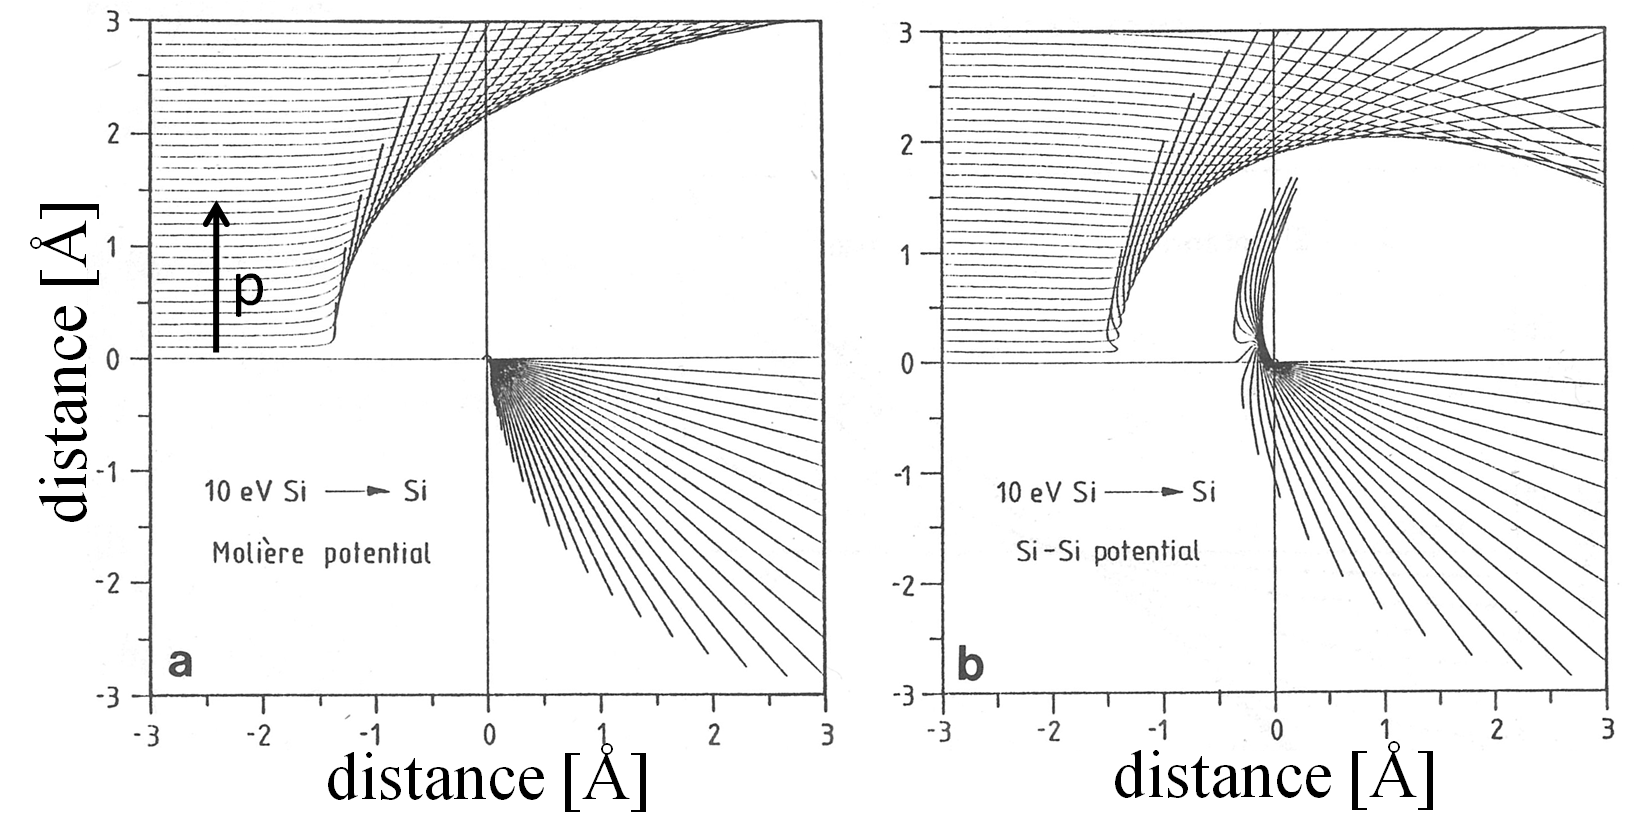
\includegraphics[width=.6\textwidth]{images/SiSicollision.png}
	\caption{Trajectories of a $10\,eV$ $Si-Si$ collision for a) Moliére and b) $Si-Si$ potential. The trajectories end after the same elapsed time for each impact parameter p. Adapted from \cite{eckstein_computer_1991}.}
	\label{SiSi}
\end{figure} 

In addition to this problem of finding the correct interaction potential for a collisions, depending on the ion and the atomic structure of the irradiated material, the collision parameters relevant to low energy collisions are within the order of the inter-atomic distance of a few \AA, see figure \ref{SiSi}. The assumption, that this is still a binary collisions can thus no longer be valid. In conclusion, it has to be noted that similar to the electronic stopping case, the assumptions for a generalized treatment of nuclear stopping are well fulfilled for large ion energies, but lose their validity at low energies $\ll\,1\,keV$.

\subsubsection{Sputtering}

A prominent role in this dissertation will be played by a special effect of nuclear energy loss arising when the path of a recoiled atom intersects the targets surface: sputtering. The foundation of sputter theory was laid by Sigmund \cite{sigmund_theory_1969}. It is outlined in the following. The nuclear stopping of ions leads to the formation of highly branched collision cascades. Therefore, the majority of recoiled atoms is found at the end of the many branches. Because of this, the majority of sputtered particles has a low energy and thus a low range in the material \cite{thompson_energy_1968}. They must thus originate from the surface of the target and the sputter yield, as the number of atoms sputtered per impinging ion, can be estimated by calculating the nuclear energy loss at the surface of the irradiated material and diving it by a factor to account for the probability of the atom leaving the solid. 

The probability for the atom to leave the solid includes geometric considerations and the `surface binding energy' (SBE). A reasonable model for the SBE is that of a potential plateau with the height of the enthalpy of sublimation which has to be overcome by the atom approaching the surface. This equates the energy required for sputtering an atom to the thermal energy required for sublimation. The SBE model for sputtering neglects all effects related to the directionality of the local binding forces experienced by the atom to be sputtered and the modification of the surface by repeated removal of atoms.

A reasonable assumption for the nuclear energy deposition distribution is be a Gaussian ellipsoid, with the center at the ion range and the longitudinal and lateral straggling naturally defining its extensions. This approach was used by Sigmund to arrive at a good explanation for the energy dependence of sputtering from flat surfaces. Starting a low energies, the sputter yield will initially increase with increasing energy, simply due to more energy being available. For further increasing energy, however, the ion range becomes larger, leading to a predominant deposition of the energy deeper inside the target, away from the surface. A maximum is thus found at energies where the ion range is in the order of the longitudinal straggling. The angle dependence of sputtering can also be explained by the increased deposition of energy near the surface for larger angles of incidence, as shown in figure \ref{anglesigmund}.

\begin{SCfigure}[50][h]
	\centering
		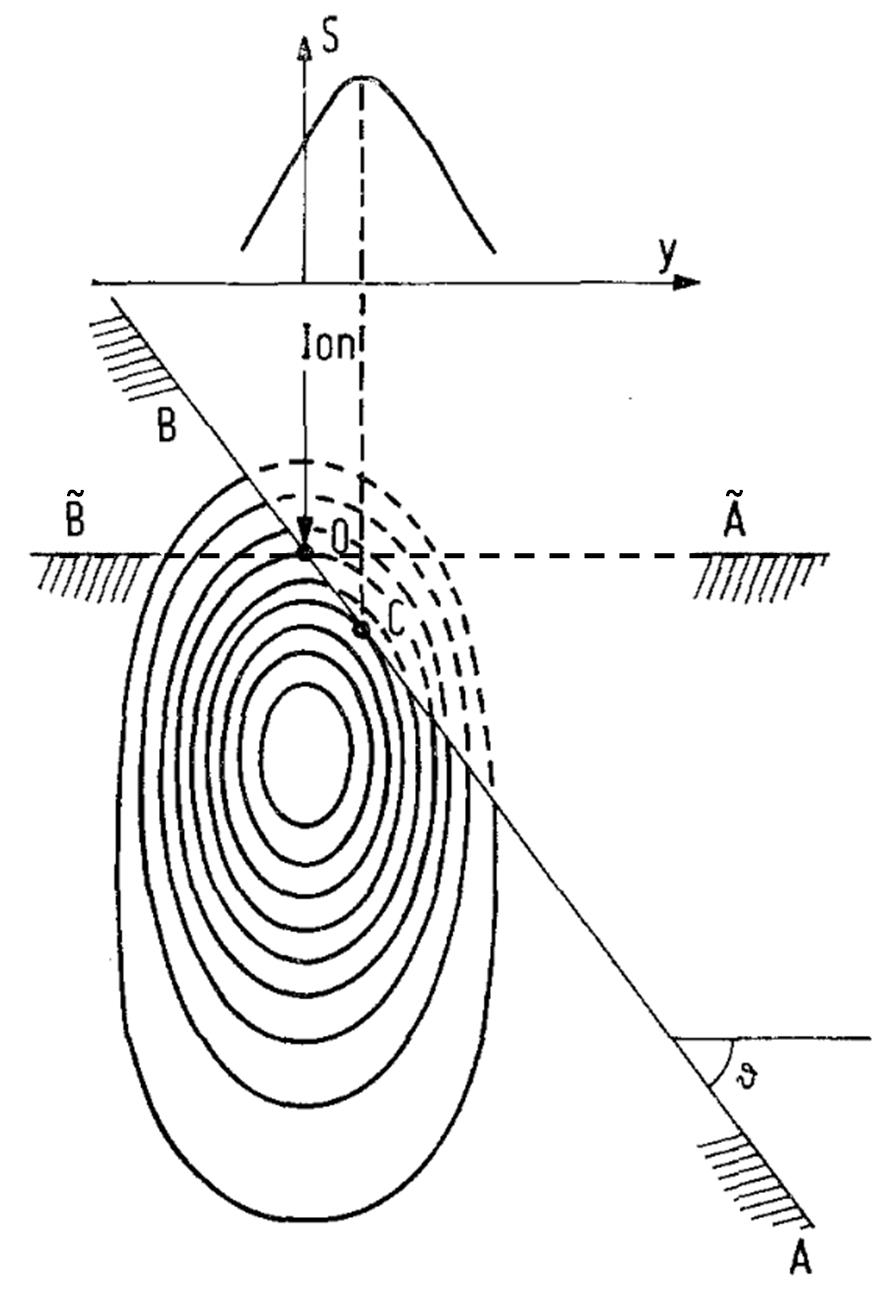
\includegraphics[width=.35\textwidth]{images/anglesigmund.jpg}
	\caption{Illustration of the Sigmund model of sputtering for irradiation of a bulk sample at an angle $\theta$. The ion enters the target at the point O and deposits the nuclear energy as indicated by the oval contours. The energy deposited along the slanted surface $BA$ is larger than that for the perpendicular surface $\widetilde{BA}$ leading to increased sputtering for irradiation at an angle. Also the deposited energy and thus sputtering is not largest exactly at the point of incidence O, but further down at the point C. This is illustrated by the projection of the sputter yield `S' onto the lateral dimension `y'.  From \cite{sigmund_mechanism_1973}.}
	\label{anglesigmund}
\end{SCfigure} 

Applications of the Sigmund theory has been made to more complex surfaces. The Bradley-Harper theory of ripple formation on ion irradiated planes relies on the anisotropic sputtering predicted by the Sigmund model applied to a structured surface \cite{sigmund_mechanism_1973,bradley_theory_1988}. The increased sputtering at a point (C) downstream from the point where the ion enters the target (O) leads to an enhancement of surface roughness.

Also recent investigations on sputtering of spherical \cite{nietiadi_sputtering_2014} and cylindrical \cite{urbassek_sputter_2015} nanostructures have found the Sigmund model to be a decent first approximation. It predicts a maximum in sputtering where the ion range is comparable to the nanostructure diameter. This can be understood by considering sputtering for a fixed ion energy and varying diameter. At large diameters atoms can only be sputtered from the surface facing the ion beam. The sputtering will still be larger than for a bulk sample as the local angle of irradiation is increased. 

For decreasing diameters the 

\section{Simulation of ion-solid interaction}

In practice the theory of ion-solid interaction is implemented in simulation tools which allow the experimenter to predict experimental outcomes. The most frequent example is obtaining the energy dependence of the ion range by simulations and using that information to decide which energy and fluence of irradiation is needed to obtain a desired doping concentration. On a deeper level, an experimentally observed behavior can be understood better by comparing it to various simulations to discern the dominating effects. The two main simulation approaches used to simulated the ion solid interaction are Monte-Carlo (MC) and Molecular Dynamic simulations (MD), both outlined in the following sections.


\subsubsection{Monte-Carlo and the binary collision approximation}

Monte-Carlo codes are simulation codes that use random numbers for simulations. After numerous simulations with different random outcomes, a statistical approximation of the likely outcome can be derived. With the BCA, the solid ion-interaction lends itself very well to MC simulation, as the evolution of a collision cascade can be simulated reiteratively by following the paths of the ion and all recoils. In the simplest case, three random numbers are needed per collision. The probability of a collision can be determined from the cross-sections determined by the interaction potential between the projectile and the atoms in the target. According to this probability, the first random number is used to determine the distance traveled in a straight line by the projectile. The particle's kinetic energy is reduced by the electronic energy loss according to the distance traveled. The underlying assumption here is that of a `random material'. Crystal structure effects such as channeling are not reproduced by this simulation. Two further random numbers are used to determine the impact parameter and azimuthal angle. The trajectories of the projectile and target atom in the plane of impact after the impact are determined by this impact parameter, the interaction potential and the particle energy. 

Examples of simulation codes implementing this approach in static planar targets are SDTrimSP \cite{bizyukov_morphology_2008}, corteo \cite{schiettekatte_fast_2008}, COSIPO \cite{hautala_nuclear_1984} and, by far the most popular, SRIM \cite{ziegler_srim_2012}. In TRIDYN \cite{moller_tridyn_1984} the target composition is `dynamic', changing with the incorporation of ions and with selective sputtering of target atoms and the incorporated ions. It is clear that the irradiation of a nanostructure can not be approximated well with a planar simulation. Therefor, for this dissertation the open source \emph{iradina} \cite{borschel_ion_2011} was extensively used. It is a BCA MC simulation run on a volume subdivided into rectangular voxels containing either vacuum or material, with the simulation volume static. The recently developed TRI3DYN \cite{moller_tri3dyn_2014} even includes dynamic composition and structural relaxation during the irradiation on a three dimensional simulation volume, but unfortunately it is not publicly available yet.

Several simulation results are of interest in this thesis. The strong point of MC BCA simulations is an accurate prediction of the distribution of the ions after irradiation. This can be expected to be upheld in the irradiation of nanowires. The concentration of incorporated ions is somewhat lower in nanowires than in bulk targets, as there are more ion paths that lead to the ions being scattered out of the wire, than just the paths leaving a planar surface \cite{borschel_ion-solid_2012}. 

Furthermore, MC BCA simulations confirm the 

Even though \emph{iradina} can implement an analytical description of a cylinder most of the simulations in this work were nevertheless performed on the voxel based simulation volume as this granted more freedom in the creation of the simulation volumes. The accuracy of the approximation of a curved surface, such as the surface of the cylindrical nanowires, is obviously dependent on the voxel size. Also, the surface and the surface of a cylinder is strictly smaller than its approximation by rectangular voxels and sputtering, as a surface effect, may be influenced. However, for voxel edges of $2\,nm$ and below only a negligible influence of the voxel size on the sputtering was found. In any case, the surface roughness of the nanowires during irradiation can be expected to be in this order of magnitude.

The accuracy of simulation results 


\subsubsection{Molecular dynamic simulations}

MD general: cite Alder, Nordlund+Kuronen


\chapter{Experimental Methods}



\section{Nanowire synthesis}

Nanowire synthesis can be categorized according to two approaches: ``bottom-up'' and ``top-down''. The ``bottom-up'' approach relies on the self-organized arrangement of matter using an inherent anisotropy in the growth mechanism to create nanoscale structures. Depending on the material, crystal quality, morphology, infrastructure requirements, the quantity to be produced etc. there is a large variety of processes available for synthesis. For semiconductor nanowires the main approaches developed are based on hydro-thermal, pyrolytic, vapor-transport, chemical vapor deposition, laser ablation, metal organic vapor phase epitaxy (MOVPE), molecular beam epitaxy (MBE) processes. 

A very common mechanism to create the anisotropy required to get the one dimensional growth of nanowires is the vapor-liquid-solid growth (VLS) first described by Wagner and Ellis. The variety of processes listed before are responsible to provide the `vapor' of material for this growth mechanism. With vapor transport the source material eg. ZnO is simply evaporated in a typically inert atmosphere and transported within an oven to the substrate by diffusion or gas flow. Chemical vapor deposition uses reactive gases such as $SiH_3$ to provide the source material, in this case $Si$ in a temperature and pressure controlled oven. Similarly in MOVPE a metal-organic gas is used as at least one of the sources. For example TMG (trimethylgallium) and $AsH_3$ to grow $GaAs$.

Although self-catalyzed growth has also been observed, the liquid part in VLS is typically played by a metal catalyst deposited on the growth substrate. The material in the vapor phase can collect in the catalyst droplet until the concentration is saturated. Preferential segregation of the nanowire material at the droplet-substrate interface leads to the growth of a wire. The size of the droplet can be used to control the diameter of the grown nanowire to some extent. $ZnO$ \cite{borchers_catalyst_2006, stichtenoth_dimensionseffekte_2008, muller_structural_2009,ogrisek_kontrolliertes_2013}, $GaAs$ \cite{borgstrom_size-_2004, wacaser_preferential_2009} and $Si$ \cite{lugstein_pressure-induced_2008} nanowires investigated in this dissertation where grown with the VLS mechanism using vapor transport, MOVPE and chemical vapor deposition respectively. An epitaxial relation between the substrate and the nanowire material may be used to direct the growth. Typical nanowire diameters and lengths are $50 - 300\,nm$ and $> 10\,\mu m$ respectively.

Nanowires can also be synthesized ``top-down''. A ``top-down'' approach requires a predefined template which is used to control the desired morphology. The $Si$-nanowire arrays investigated within this dissertation were etched by reactive ion etching (RIE) through a circular, e-beam lithographically defined $Ni$ hard-mask which set the nanowire diameter \TODO{cite NL}. With the ``top-down'' etching process it is possible to prepare nanowires with diameters varying from $50\,nm$ to $2\,\mu m$ with a height of $\approx 3\mu m$ on a single substrate for simultaneous irradiation. 

Since the growth of nanowires was performed mainly by collaborators in Lund University ($GaAs$) and TU Vienna ($Si$) and is not part of the investigations reported here, the inclined reader is redirected to the the cited references for further details respective growth parameters and their investigation.

\section{Modification}


\subsubsection{ROMEO}


The ion irradiation for this dissertation was performed at the general purpose HVE implanter ``ROMEO'' at the IFK in Jena. It can provide an ion beam of virtually any element at energies of $10-380\,keV$. The beam passes a $90^\circ$ selector magnet and can be sweeped with a frequency of $kHz$ to homogeneously irradiate areas up to several tens of $cm^2$ with ion currents of up to $1\,mA$. For this work ion current densities were limited to $500\,nA/cm^2$ or $10^{16}\,ions/cm^2$ in $15\,min$. As previous work has shown that the irradiation of nanowires can bend the nanowires \cite{borschel_permanent_2011, borschel_ion-solid_2012}, a rotatable and heatable, tilted stage (RHT) was custom built \cite{noack_sputter_2014}. With it, bending of the nanowires that are upstanding on a substrate can be avoided as they are irradiated homogeneously from all sides at an angle of $45^\circ$. All the samples investigated in this thesis were rotated on the RHT and its preceding prototype sample stages during the irradiation. 
%RHT Bild?

\subsubsection{FIB}

%hier ist noch blabla drin:
Some sample preparation required a focused-ion-beam (FIB). FIBs are highly specialized ion accelerators where the main objective is to obtain a small ion beam focus. The most wide spread systems use a $Ga^+$ beam and acceleration voltages up to $30\,keV$. The main use for FIBs is to use the focused ion beam to sputter material extremely locally, making it a versatile tool for nano-machining. The FEI DualBeam Helios NanoLab 600i FIB system used for this dissertation is a scanning electron microscope (SEM) - FIB combination, so that the sample can be milled with the ion beam and investigated with the SEM. It also is equipped with a $Pt$-metal-organic-gas injection system. The $Pt$ containing organic gas can be cracked locally on the sample by the secondary electrons created by either the electron or the ion beam. The FIB system can thus deposit and mill structures on a $nm$ scale. For the sample preparation in this thesis all $Pt$ deposition was done with the electron beam. Most of the $Pt$ is deposited near the impact point of the primary beam and the substrate, however typically a rather large `halo' of minor $Pt$ deposition can extend for a couple of $\mu m$. 

\section{Characterization}

\subsubsection{SEM}

The morphological changes in the nanowires were characterized by high resolution SEM in the FEI DualBeam Helios NanoLab 600i focused-ion beam system. The spacial resolution of the SEM system is $\approx 2\,nm$. To quantify the sputtering, images of individual nanowires were made before and after ion irradiation. To find exactly the same place on the sample, a series of images with increasing magnification has to be made. Typically images were made at an angle of $45^\circ$ to the substrate with the substrate aligned the same way before and after irradiation.

An semi-automated image analysis protocol was developed by Stefan Noack in his Master thesis \cite{noack_sputter_2014, NL} to evaluate the SEM images of a large number of nanowires. It applies a (3x3) median filter to smoothe out some noise and a Gaussian unsharp mask with $\sigma = 1\,px$ and weighted at $60\,\%$ to resharpened the edges \cite{sankur_survey_2004}. An Otsu thareshold \cite{otsu_threshold_1979} is applied to separate the lighter nanowire from the darker background. Next, open source particle analysis software is used to find the main body of the nanowire and turn the it upright, correcting for any marginal tilt remaining in the SEM images \cite{schindelin_fiji:_2012,sage_imagej_2012}. Finally the sum of the gray-values in each line used to calculate the diameter at that height along the nanowire axis. As the investigated nanowires showed a characteristic bulge at the base, this point can be used to align the height profiles of a single wire before and after irradiation.

\subsubsection{EBSD}

Electron back-scatter diffraction (EBSD) was used to identify whether nanowires remained crystalline after irradiation with a Carl Zeiss Auriga CrossBeam Workstation. EBSD can be measured with a large CCD detector in a SEM. The electron beam is focused on the sample at an arbitrary angle. Electrons are scattered from the sample lattice and the scattered electrons are detected by the CCD detector. Bragg diffraction along the crystal lattice planes produces a characteristic pattern of Kikuchi lines on the detector \cite{kikuchi_diffraction_1928,fultz_transmission_2013} in crystalline samples. Amorphous or nano-crystalline samples show no pattern.

\subsubsection{nano-XRF}

The most experimentally advanced characterization method was X-ray fluorescence with a nano-focussed X-ray beam (nano-XRF) at the European Synchrotron Radiation Facility (ERSF), beamlines ID16b and ID13. Hard X-ray radiation excite the atoms within a radiated material to emit characteristic X-ray radiation. This X-ray fluorescence can be detected in an energy dispersive semiconductor detector and used to identify and quantify the elements in the sample. In principle the method is similar to the more wide-spread energy dispersive X-ray spectroscopy (EDX), where an electron beam is used to excite characteristic X-ray fluorescence. Very good lateral resolution can be obtained by having an EDX detector in an SEM. The advantage of using X-rays lies in the absence of Bremsstralung which high energy electrons in matter produce in addition to characteristic X-rays. In XRF there is thus a much lower background and much lower concentrations of elements can be detected and quantified. Unlike normal X-ray tubes, synchrotron radiation is very brilliant, allowing it to be focused. The beamlines ID16b and ID13 were run at various energies above $16\,keV$ and a focus of typically $\approx 80\,nm$ and $\approx 250\,nm$ respectively. The nano-XRF thus allows for quantification of low concentrations with sufficient lateral resolution to resolve axial concentration gradients in a nanowire. Unfortunately, the resolution is not good enough to investigate radial distributions.

At both beamlines the nanowires are scanned under the fixed focal point of the X-ray beam with piezo-motors while the XRF spectra are collected with a Vortex EM silicon drift X-ray detector. The investigated $Mn$ irradiated $ZnO$ nanowires were deposited on TEM grids either randomly by `imprinting' or individually by using the mico-manipulator in the FEI DualBeam FIB. Transferring individual wires requires some finesse, but it is possible to detach the $ZnO$ nanowires from their substrate without the $Ga$ FIB and to place them on the ``lacey-carbon'' TEM Grids without any additional $Pt$ deposition. In this way SEM images before and after irradiation of the same wire investigated by nano-XRF are available.

The spectra used for quantification were obtained in multiple scans across a nanowire at regular intervalls along the nanowire's length. As the XRF signal can be used to locate the nanowire, only the points near the nanowire were measured with a high integration time and a low step-with ($< \frac{1}{2}$ focal spot) to ensure a large number of counts ($> 10^5$ per scan) at reasonable measuring times.

\subsubsection{nano-XRF quantification}

The XRF-Spectra were evaluated using the open source PyMCA software package \cite{sole_multiplatform_2007}. The effects of self absorption and excitation can be neglected, as the investigated nanowires are very thin compared to the absorption length of a couple of $\mu m$ of hard X-rays in $ZnO$. However, the detector-sample distance is an unavoidable attenuation length in air, in which the X-ray absorption is dominated by $Ar$. As the element investigated, $Mn$, is relatively light, its characteristic X-ray emission at $K_{\alpha,Mn} = 5.9\,keV$ suffers more absorption than the heavier $Zn$ with $K_{\alpha,Zn} = 8.6\,keV$. Thus absorption of the XRF signal in air has to be considered carefully in the fitting with PyMCA. The accuracy was double checked by measuring and quantifying trace elements in a calibration sample of bovine liver. In this way optimal fitting parameters were found for each beam-time and applied to the respective spectra in the PyMCA batch mode.  Oxygen can not be quantified in these beamlines, as its XRF emission is totally attenuated by the air and a $Si$ dead layer in the detector. The quantification of the $Mn$ content in the $ZnO$ nanowires thus relies on the assessment of the $Mn/Zn$ ratio. It a decent approximation to assume that the $ZnO$ remains stoichiometric even during the irradiation. The samples are irradiated in a chamber with a base pressure $\approx 10^{-6}\,mbar$, so according to the Hertz-Knudsen equation this will give a coverage of roughly one mono-layer or $10^{15}\,particles/cm^2s$. The maximum ion current density of $500\,nA/cm^2s$ amounts to $10^{13}\,ions/cm^2s$, so that an unlikely amount of preferential sputtering would be required to deplete the oxygen out of the wires. In any case, the wires will be oxidized in the normal atmosphere post irradiation. The $Mn/Zn$ ratio is thus a good proxy for the $Mn$ concentration.

The quantification limit can be tested within PyMCA by finding an appropriate photon flux and nanowire interaction volume for a simulation to reproduce the XRF spectrum with the actually measured number of counts at $K_{\alpha,Zn}$. The $Mn$ content in the simulated matrix can then be decreased until the minimum $Mn$ content is found which gives a signal at $K_{\alpha,Mn}$ just above the actually measured noise level. In this way a lower limit for the concentration resolution can be found at typically $0.1\,\%\,Mn/Zn$.





%\chapter{Sputtering of Nanowires}
\label{sec:sputter}

The experiments presented in this chapter were conducted together with Stefan Noack and are partially published in his master thesis \cite{noack_sputter_2014} and in reference \cite{johannes_anomalous_2015}.

% \section{First results in $Mn$ irradiated $GaAs$}

% Introduction by Mn in GaAs (JPhysD)


\section{Simulation of the sputter yield}
\label{sec:simsputering}

The sputtering of nanowires can be investigated by MC simulations using the software \emph{iradina}. The discussion of the Sigmund sputter model in Chapter \ref{sec:ionsolid} concluded that a maximum is expected for a certain ion species, ion energy and nanowire diameter combination. This is confirmed by MC simulations for the examples of $Xe^+$ (Figure \ref{sputtering_de}a) and $Ar^+$ (Figure \ref{sputtering_de}b) ions, respectively. A $Si$ nanowire is irradiated homogeneously at an angle of $45^\circ$ between the nanowire axis and the ion beam. In multiple simulations, the nanowire diameter and ion energy were both varied. The white line indicates the ion range of the respective ion in bulk, as calculated with SRIM and projected on to $45^\circ$. The maximum of the sputtering correlates very well with this ion range for both ion species. The heavy $Xe^+$ naturally has a much lower ion range than $Ar^+$ at the same ion energy. Also, sputtering is larger by about a factor of $2.5$ for the denser collision cascades caused by the heavier $Xe^+$ ions.

\begin{figure}[th]
	\centering
		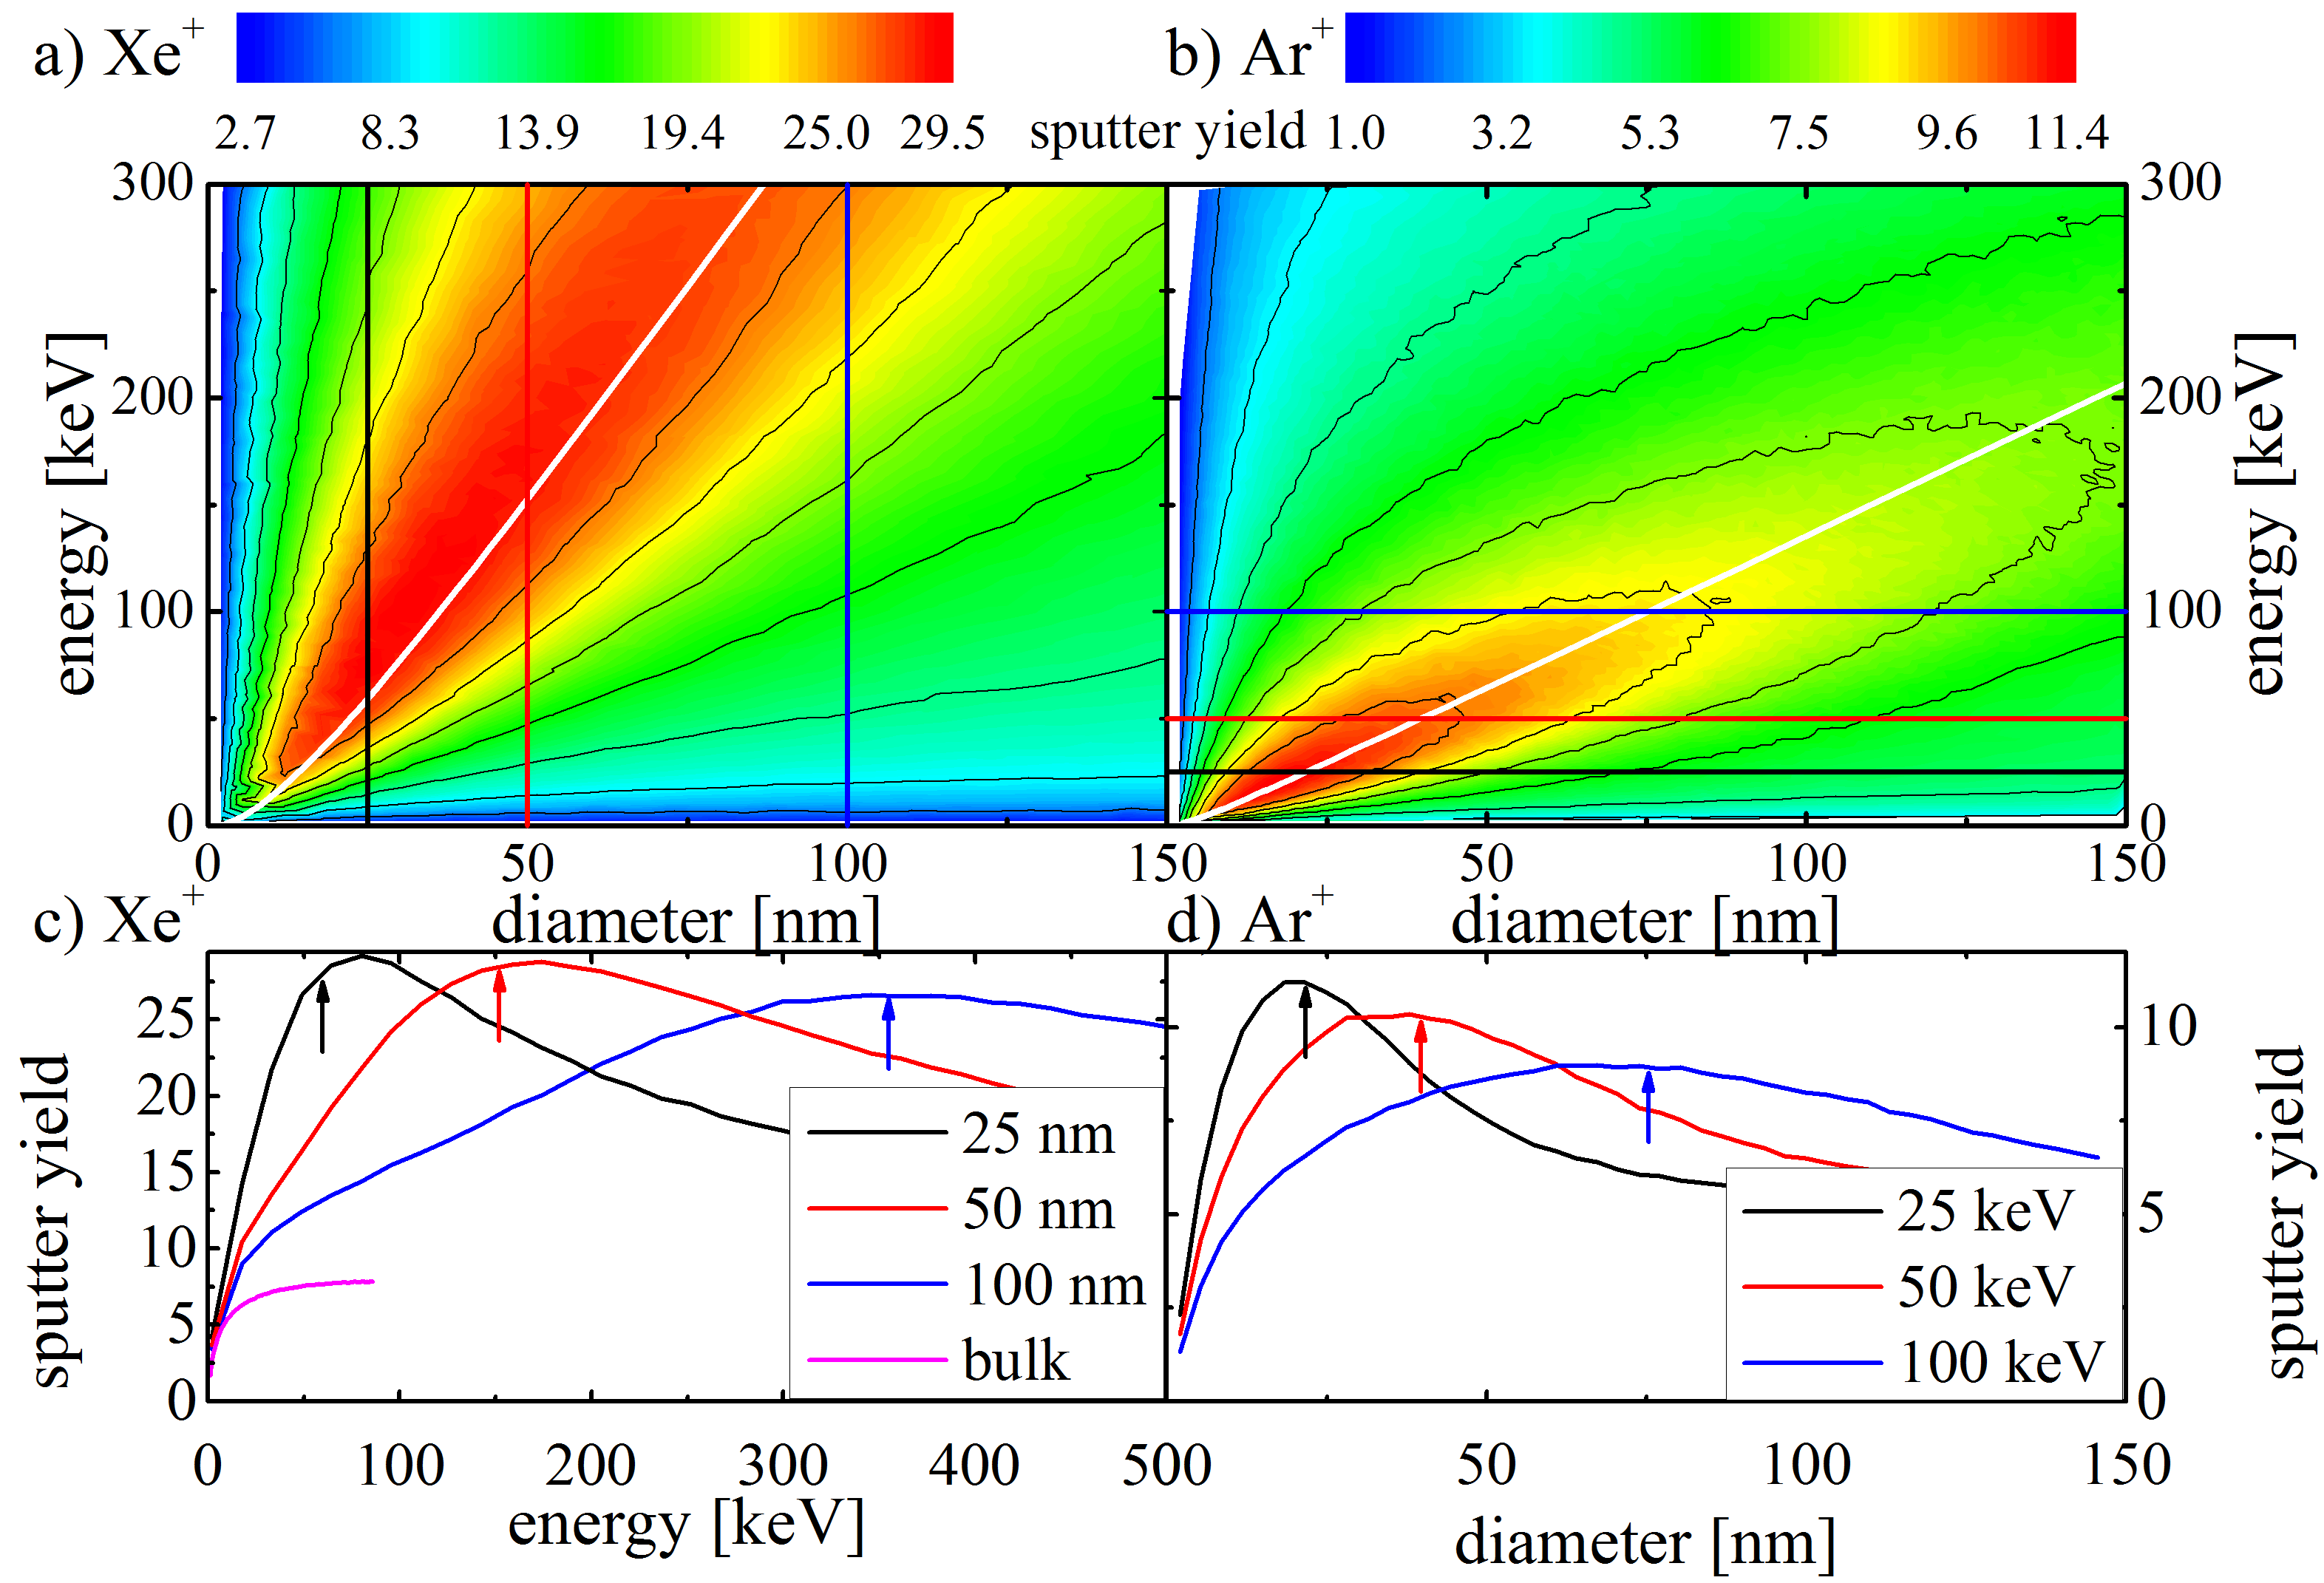
\includegraphics[width=.9\textwidth]{images/sputtering_diameter_energy.png}
	\caption{Contour plot of the sputter yield simulated with \emph{iradina} for the irradiation with $Xe^+$, a) and $Ar^+$, b) ions of varying energy into $Si$ nanowires with varying diameters. The white lines indicates the respective ion's range in $Si$ bulk at $45^\circ$, calculated with SRIM. The vertical lines in a) and horizontal lines in b) indicate where the sputter yields for a set of constant diameters c) and constant energies d) was extracted. In c) and d) the ion range in bulk is indicated with colored arrows.} 
	\label{sputtering_de}
\end{figure} 

In \ref{sputtering_de}c, the sputter yield versus ion energy is extracted from the $Xe^+$ simulation for a set of fixed diameters. The black, red and blue curves correspond to the simulation of $25, 50$ and $100\,nm$ diameter wires, respectively. The corresponding vertical lines in Figure \ref{sputtering_de}a show the position of the extracted data in the contour plot. The maximum clearly shifts to larger ion energies for larger nanowire diameters. The colored arrows indicate the ion energy for which the ion range, simulated by SRIM, is equal to the respective diameter. The magenta curve shows the energy-dependent sputter yield for a flat $Si$ surface irradiated with $Xe^+$ ions at $45^\circ$, simulated with \emph{iradina}. The broad maximum sputter yield for this bulk simulation is found at $\approx 100 \,keV$. Correspondingly the global maximum sputter yield in nanowires is also found at $\approx 100 \,keV$ for $\approx 30\,nm$ diameter wires.

The sputter yield from $Ar^+$ irradiated $Si$ nanowires is plotted as a function of the diameter for a set of fixed energies in Figure \ref{sputtering_de}d. Here, the black, red and blue curves correspond to $25, 50$ and $100\,keV$ ions and the arrows indicate the ion range at the respective energy. Again the maximum sputtering is found at a diameter corresponding to the ion range in bulk.

To relate this to the Sigmund sputtering model, with its Gaussian ellipsoid approximation of the damage profile, a Gaussian peak can be fitted to the recoil profile simulated with SRIM for both ions in $Si$ \cite{bobes_ion_2012}. The so found mean damage depth is constantly found at approximately $0.7$ times the ion range for the whole energy range investigated here. A naive, first approximation with the Sigmund sputtering model would predict that the sputtering is maximal where the ions energy is such, that the mean depth of the damage and the radius of the irradiated nanowire coincide. However, this is only true for central impacts, while the simulated situation is an average over all ion-nanowire impact parameters. For non-central impacts there is less of the nanowire `in front' of the ion's path. Therefore, the maximum of the sputter yield is also at lower energies than it would be for solely central impacts. It is thus a consequence of the irradiation geometry that the diameter of maximum sputtering is equal to the projected ion range and not the mean depth of the damage distribution. To test the limits of the Sigmund model, a more thorough investigation of the Sigmund model's predictions for various irradiation scenarios may be interesting; however, because the MC simulations reproduce the reality more realistically anyhow, it will not be undertaken here.


\vfill
\section{Redeposition}
\label{sec:redeposition}

While irradiating a nanowire which is standing perpendicular on a substrate, as is the case in the samples shown in Figure \ref{SEMarray}, material will also be sputtered from the substrate. Some of the sputtered material from the substrate will be redeposited on the nanowire, so that the observable sputter yield will be lower than the actual sputtering from the nanowire. The following calculation will estimate how many atoms are redeposited on the nanowire per irradiated ion fluence on the substrate. Consider the situation shown in Figure \ref{redeposit}. An ion hits the substrate at point \emph{A}. A possible path of a sputtered atom is indicated by the red line to a point on the nanowire, where the substrate atom is redeposited on the nanowire. 

\begin{SCfigure}[][b]
	\centering
		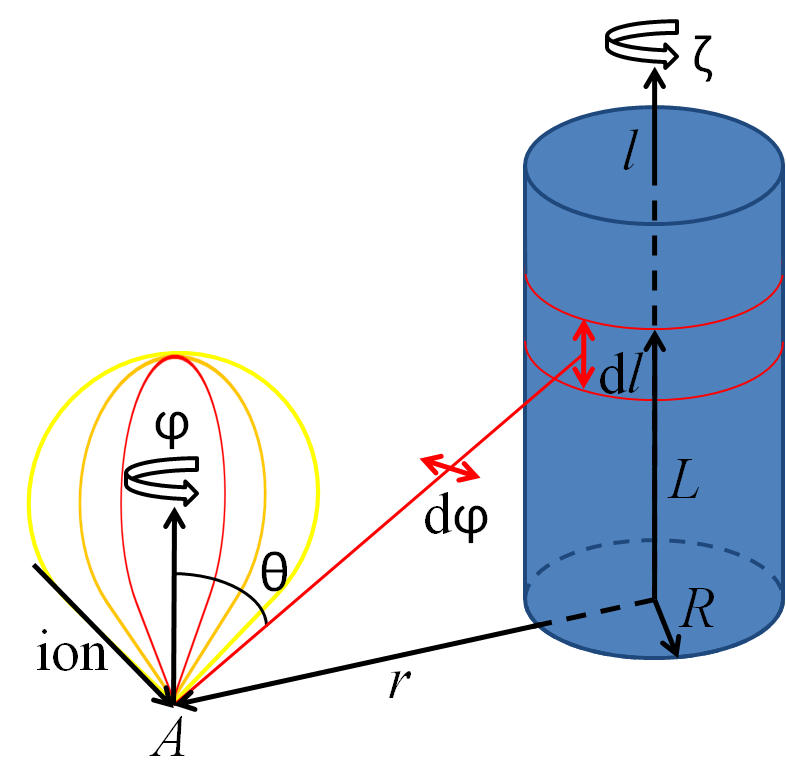
\includegraphics[width=.45\textwidth]{images/redeposit.jpg}
	\caption{Illustration of the redeposition of sputtered material from the substrate point \emph{A} onto the nanowire with radius \emph{R} at a height \emph{L}. Because the wire is rotated around its axis $\zeta$ and the whole substrate is irradiated, a rotationally symmetric angle distribution for the sputtered atoms can be chosen.} 
	\label{redeposit}
\end{SCfigure}

First, the probability $P$ of a sputtered atom to hit the nanowire is calculated:

\begin{equation}
\label{prob1}
P = \int_0^{2\pi} \! \,\int_0^{\pi/2} \!\! H(\theta,\varphi,r,R,L) \, \tilde{SY}(\theta,\varphi) \,cos(\theta)\,\mathrm{d}\theta \, \mathrm{d}\varphi,
\end{equation}

where $H(\theta,\varphi,r,R,L)$ is the probability distribution of hitting the nanowire. It is normalized to the inverse of the total solid angle \nicefrac{1}{$4\pi$}, if the trajectory along $\theta$ and $\varphi$ from $A$ hits the nanowire with length $L$ and radius $R$, and zero otherwise. For irradiation at an angle, the angle distribution of the sputter yield $\tilde{SY}(\theta,\varphi)$ is expected to have a preferential direction along the ion beam \cite{verdeil_angular_2008}. However, the effective distribution becomes rotationally symmetric (independent of the angle $\varphi$) if one neglects the shadowing of the ion beam on the substrate by the nanowire. Then, all points around the wire are hit, and the wire is rotated around its axis (angle $\zeta$), so that an effective, rotationally symmetric angle distribution $\tilde{SY}(\theta)$ of the sputtered atoms from the substrate can be used, as indicated by the yellow, orange and red bulbs in Figure \ref{redeposit}. A $cos^\kappa(\theta)$ distribution is chosen: 

\begin{equation}
\tilde{SY}(\theta) = \frac{SY \cdot cos^\kappa(\theta)}{\int_0^{2\pi} \! \mathrm{d}\tilde\varphi \,\int_0^{\pi/2} \! cos^\kappa(\tilde\theta) cos(\tilde\theta)\,  \mathrm{d}\tilde\theta} \, = \frac{SY}{c(\kappa)} \cdot cos^\kappa(\theta) ,
\end{equation}

where the denominator $c(\kappa)$ normalizes the angle distribution function $cos^\kappa(\theta)$ and $SY$ is the total sputter yield from the surface. Because it forms a flattened angle distribution for $\kappa < 1$, this increased emission of atoms at larger angles $\theta$ can emulate the rotation of a slanted angle distribution.

The parametrization of $H(\theta,\varphi,r,R,L)$ in $\varphi$ is straightforward, because the integration bounds for $\varphi$ are $[-\gamma, \gamma]$ with $\gamma = arcsin(R/r)$ the angle between $r$ and the tangent to the nanowire in Figure \ref{anglesredepo}a. To solve the integration over $\theta$, it is useful to express the distance $q$ from the impact point to the base of the nanowire as a function of $\rho = R/r, r$ and $\varphi$:

\begin{equation}
q(\rho,r,\varphi) = r\cdot \sqrt{1 + \rho^2 - 2sin^2(\varphi) - \sqrt{cos^2(\varphi)(cos(2\varphi) - 1 + 2\rho^2)}}.
\end{equation}

\begin{figure}
	\centering
		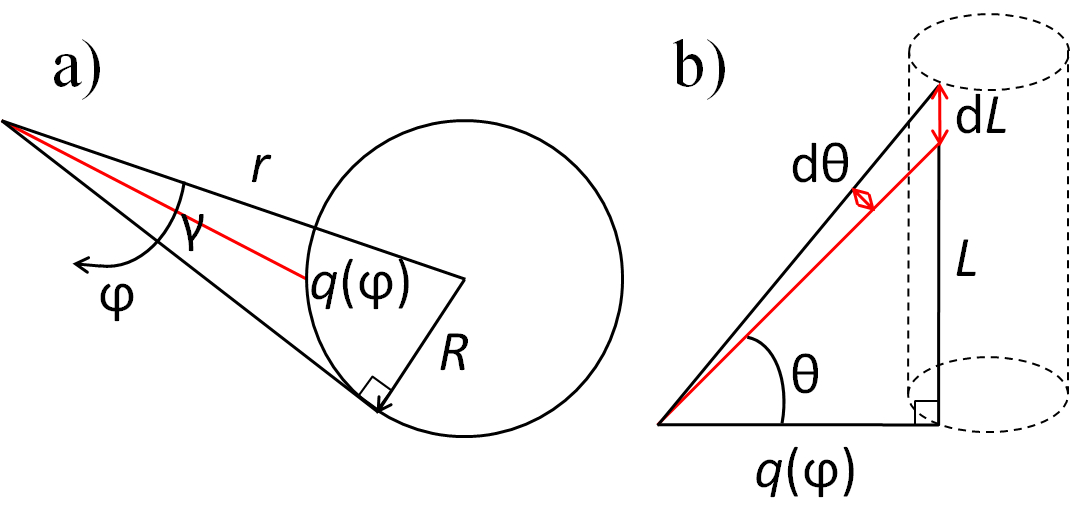
\includegraphics[width=.7\textwidth]{images/anglesredeposition.jpg}
	\caption{a) Top view: $R$ is the radius of the nanowire, $r$ the distance from the point of impact A to the center of the wire and $q(\phi)$ the distance to the wire's surface at the base of the wire. The angle between $r$ and the tangent to the nanowire circumference is $\gamma$. b) Side on view: $\theta$ is the angle between the substrate normal and the trajectory of a sputtered substrate atom to hit the wire at $L$.} 
	\label{anglesredepo}
\end{figure} 

Then the integration over $\theta$ can be substituted by an integration over the length of the nanowire $l$. The substitution can be found looking at Figure \ref{anglesredepo}b:

\begin{align*}
\mathrm{d}\theta &= \frac{sin(\theta)}{\sqrt{L^2 + q^2}}\,\mathrm{d}L,\\
\theta &= arctan(q/L).
\end{align*}

Inserting into equation \ref{prob1} and simplifying yields:

\begin{equation}
\label{prob2}
P = \frac{2\,SY}{c} \int_0^{\gamma} \! \int_{L_1}^{L_2} \!  \frac{l^{\kappa+1}\,q}{(l^2 + q^2)^{(\kappa + 3)/2}} \,\mathrm{d}l \, \mathrm{d}\varphi.
\end{equation}

With $l^*=L_1-L_2$, the area hit on the nanowire is now $\pi \, R \, l^*$, positioned at the height $L= (L_1+L_2)/2$ as indicated between the two red lines in Figure \ref{redeposit}. Next, the probability $P$ to hit the nanowire at each substrate position is integrated over the whole substrate area and normalized to the area of the nanowire which is hit. This yields the fluence of atoms $\Theta$ hitting the nanowire at height $L$ per irradiated ion fluence $\Phi$:

\begin{equation}
\label{prob3}
\frac{\Theta}{\Phi} = \frac{2\,SY}{c \pi Rl^*} \int_0^{2\pi}\! \mathrm{d}\zeta \int_R^{\infty} \!
\int_0^{\gamma} \! \int_{L_1}^{L_2} \! r \frac{l^{\kappa+1}\,q}{(l^2 + q^2)^{(\kappa + 3)/2}}\,\,\mathrm{d}l \, \mathrm{d}\varphi\,\mathrm{d}r.
\end{equation}

The integration can be solved using the numerical integration tools CQUAD and QAGI \cite{gough_gnu_2009}. Perhaps counter-intuitively, the result is independent of the nanowire radius $R$ and the height $L$ for which the deposition is calculated. For the generous estimation of a very broad distribution with $\kappa = 0.25$, the redeposition amounts to only $\Theta =10\,\% \cdot \Phi\cdot SY$. As already shown in Figure \ref{sputtering_de}c, the sputter yield is significantly lower from the plane substrate than from the nanowire. Therefore, the redeposition can be safely neglected for the evaluation of sputtering. However, redeposition may remain relevant to substrates of a different material than the nanowire, if the incorporation of substrate atoms in the nanowire has detrimental doping effects. Because the atoms redeposited from the substrate have a very low energy, they will be deposited on the surface of the nanowire. This position at the surface of the nanowire makes them prone to re-sputtering, which reduces the finally incorporated number of substrate atoms further. Nevertheless, keeping the redeposition in mind is advised in choosing the substrate material.


% However, this can be made plausible by looking at Figure \ref{anglesredepo}. There is no characteristic radius $R_c$ which would change any of the geometric relations in \ref{anglesredepo}a. Since the integration is over all the $r > R$, necessarily always starts at $P(R) =1/2$ and goes to $P(r\rightarrow \infty) =0$, its result is independent of $R$. For $L$ it can be argued in Figures \ref{anglesredepo}b or \ref{redeposit} that for a fixed $\theta$, $\mathrm{d}L \propto 1/r$ scales as the inverse of the area $\mathrm{d}A \propto r$ of the annulus radiating towards the nanowire under that angle. Therefore the redeposition is constant along the whole nanowire length. 




\section{Si nanowire sputtering by Ar$^+$ irradiation}
\label{sec:sisputtering}

The experimental verification of the diameter-dependent maximum in sputtering was investigated on etched $Si$ nanowire arrays. Figure \ref{sputtering_exp}a shows the principle irradiation setup illustrated by a SEM image of a single nanowire before and after the irradiation with $300\,keV\,Ar^+$. The etched nanowire samples and the RHT allowed the simultaneous, rotated irradiation of upstanding nanowires with various diameters at $300\,^\circ C$. Figure \ref{sputtering_exp}b shows the extracted and aligned diameter versus height profile for the nanowire in Figure \ref{sputtering_exp}a. More than a hundred such profiles were semi-automatically extracted for many different nanowire diameters from SEM images made before and after two separate ion irradiation steps with an ion fluence of $2\cdot10^{16}\,\nicefrac{ions}{cm^2}$. The sputter yield calculated from these extracted profiles is plotted versus the local diameter in \ref{sputtering_exp}c for $100$ and $300\,keV\,Ar^+$.

\begin{figure}[th]
	\centering
		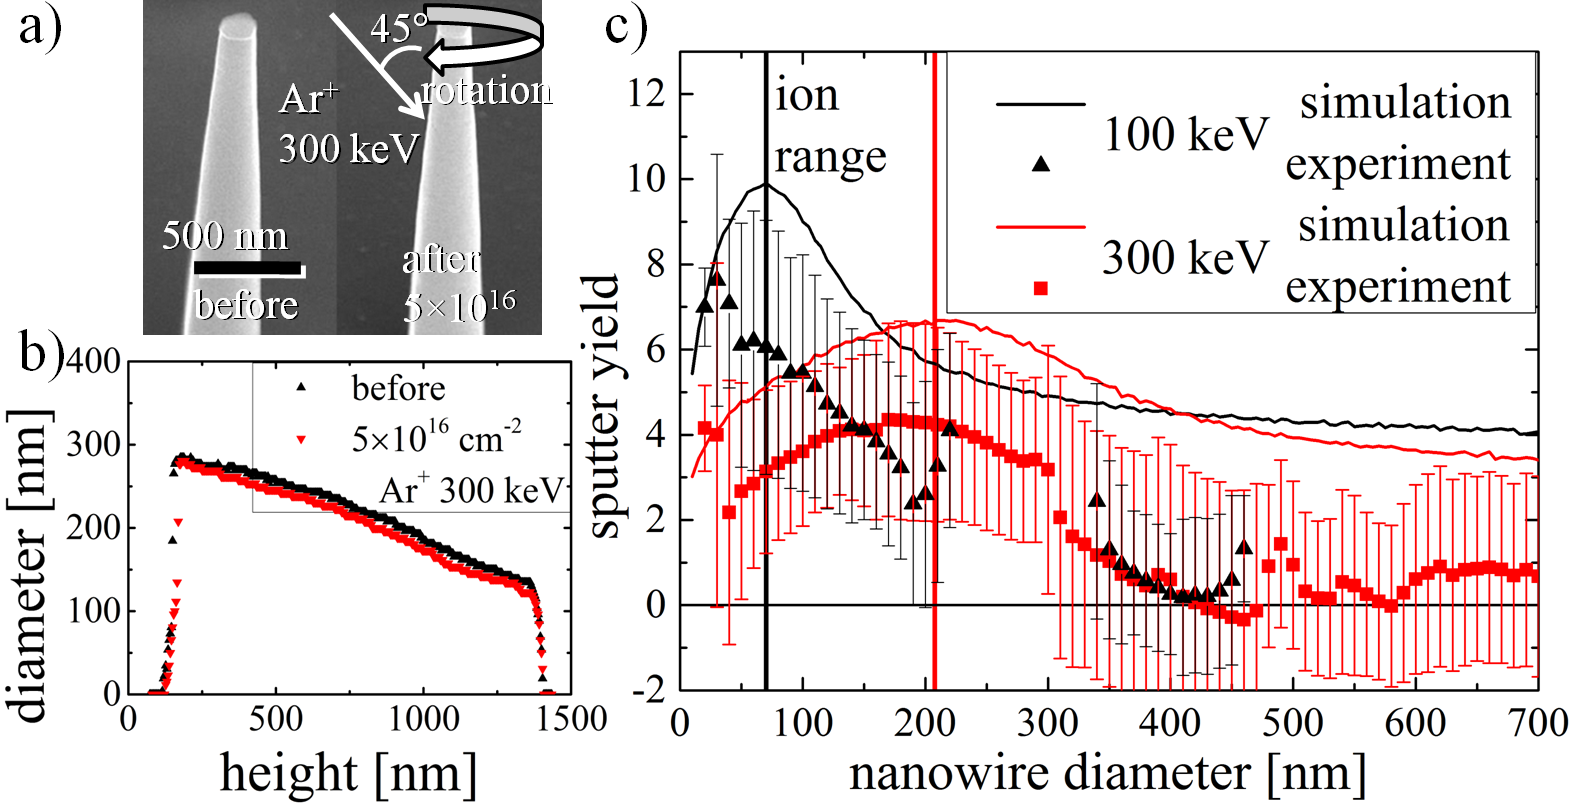
\includegraphics[width=.95\textwidth]{images/sputter_exp.png}
	\caption{a) Exemplary SEM images of a $Si$ nanowire before and after the rotated irradiation with $300\,keV\,Ar^+$ at $300^\circ C$. The extracted diameter vs. height profile for this nanowire is shown in b). From many such profiles the sputter yield vs. diameter was calculated and plotted in c) as black triangles and red squares for the irradiation with $100$ and $300\,keV\,Ar^+$, respectively. The `error bars' indicate the variance of the data points grouped together every $10\,nm$. The sputter yield calculated with \emph{iradina} simulations is shown for either case as a line-plot. The corresponding SRIM ion range at $45^\circ$ is marked by a vertical line.} 
	\label{sputtering_exp}
\end{figure} 

The experimental sputter yield reproduces the qualitative, simulated diameter dependence of the sputter yield well. The experimental values are, however, lower than the simulation results by $2$-$4$ \nicefrac{atoms}{ion} in absolute sputter yield or roughly a factor of 2. For $100\,keV\,Ar^+$ ions the sputter yield is largest in $\approx 60\,nm$ diameter nanowires and decreases quickly with increasing diameters. With $300\,keV\,Ar^+$ ions a broader maximum arises at diameters of $\approx 170\,nm$. For both ion energies, the maximum sputtering is found for those nanowire diameters, where the diameter is similar to the ion range, just as discussed in Chapter \ref{sec:simsputering} and the Sigmund sputtering model in Chapter \ref{sec:ionsolid}.   

The fact that the experimentally observed sputter yield has its maximum at slightly lower diameters than the simulated values for both the $100\,keV$ and $300\,keV$ irradiations may indicate the occurrence of cluster and thermal sputtering. Both have been predicted with MD simulations \cite{nietiadi_sputtering_2014,urbassek_sputter_2015,anders_sputtering_2015}, albeit in nanostructures with much smaller dimensions. This can shift the maximum sputter yield toward smaller diameter nanowires, because the kinetic energy of the ion is, on average, distributed to fewer atoms in nanowires with smaller diameters, so that both cluster and thermal sputtering increase for decreasing nanowire diameters.

The interruptions and discontinuities for diameters $<50\,nm$, at $\approx 200\,nm$, $\approx 300\,nm$ and $\approx 500\,nm$ are located where the diameter range of an array of nanowires on the irradiated substrate ended. Here, there are fewer (none for 100\,keV at $\approx 200 - 300\,nm$) nanowires which could be evaluated. The large variance indicated in Figure \ref{sputtering_exp}c as `error-bars' can be attributed to the relatively small observed diameter changes of approximately $5\,nm$, which are close to the resolution limit of the SEM at $2\,nm$. Therefore, the observation of a reasonale sputter yield value for one diameter is only possible with the large sample number, $>1000$. This problem could be reduced by increasing the ion irradiation fluence step size, so that there is a larger difference between the nanowire diameters before and after ion irradiation. However, this would invariably increase the variance in the mean diameter for which the sputter yield is determined. Before the irradiation, an approximation using the simulated sputter yields was made to find an optimum ion fluence step size, but with the low sputter yield observed in the experiment the chosen ion fluence steps of $2\cdot10^{16}\,\nicefrac{ions}{cm^2}$ are on the low side.

Sputter yields of around $0\,\nicefrac{atoms}{ion}$, as found in the experimental values at $400\,nm$, are not realistic. They have to be attributed to misalignment and remaining focal plane, brightness and contrast differences between the SEM images before and after irradiation, which could not be corrected in the image analysis. These differences introduce systematic deviations, which may be different from one nanowire array to the next. Therefore, the variance is a more sensible estimation for the overall accuracy of the experimentally determined sputter yield than the more usual standard deviation. Because of the large number of investigated nanowires, the standard deviation is so small that it would disappear behind the data points in the graph and overestimate the actual experimental accuracy considerably.

\begin{SCfigure}[50]
	\centering
		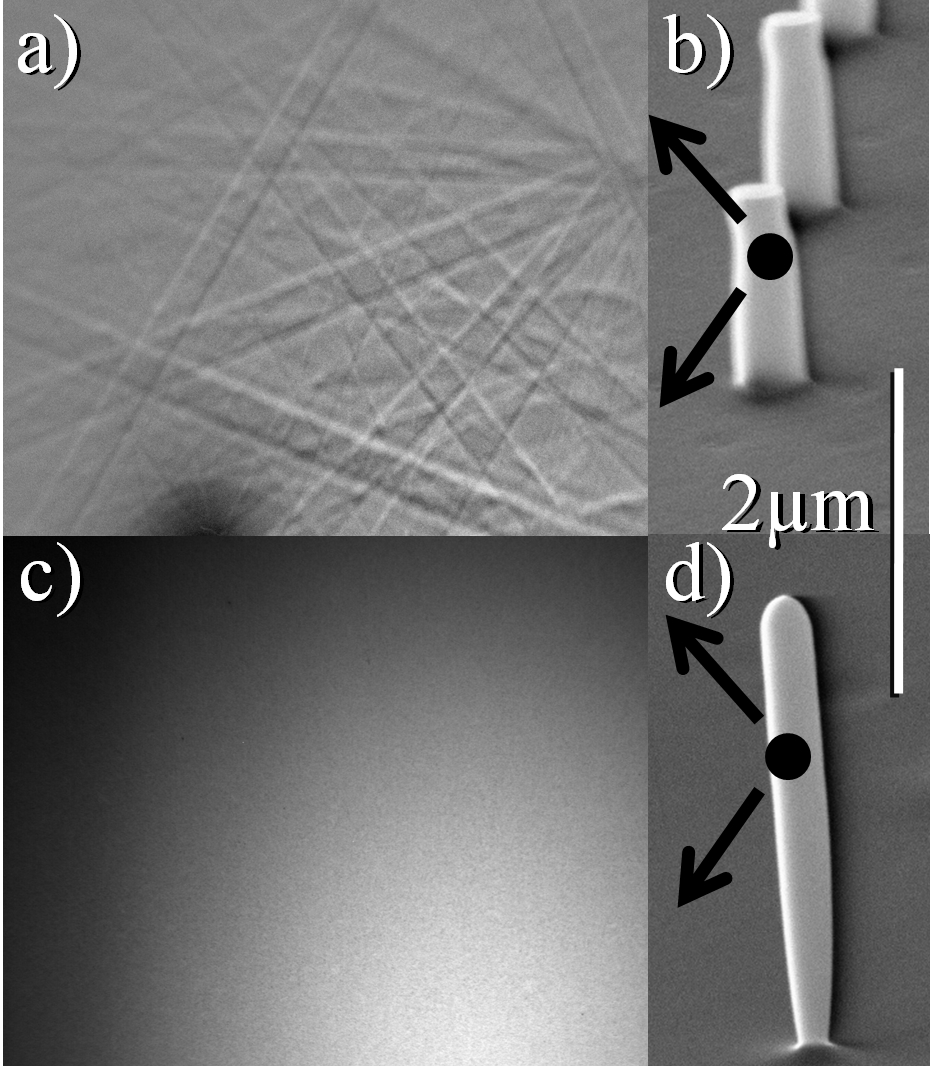
\includegraphics[width=.35\textwidth]{images/EBSD.jpg}
	\caption{The Kikuchi pattern a) clearly shows that the nanowire, shown in the SEM image b), has remained crystalline during the irradiation at $300^\circ C$. The lack of any structured signal in c) shows that the nanowire irradiated at room-temperature, shown in the SEM image d), was amorphized.} 
	\label{EBSD}
\end{SCfigure}

The quantitative discrepancy between the simulated sputter yield and the experimental values is not unexpected. To start with, the quantitative value from the \emph{iradina} simulation is questionable (Chapter \ref{sec:simion}). In the experimental values, any effect of incorporated defects, or even amorphization, on the density of the $Si$ in the nanowires can be confidently discarded, because nanowires remained crystalline during the irradiation even up to the high fluence of $5\cdot 10^{16}\,cm^2$. This was expected from irradiation studies found in literature \cite{pelaz_ion-beam-induced_2004} and confirmed by EBSD (Figure \ref{EBSD}). The main contribution to a systematic deviation in the experimentally evaluated sputter yields is the oxidation of the $Si$ nanowires in air between the subsequent irradiation and SEM investigation steps. The thickness of oxidized $Si$ on the surface of the nanowires is dependent on uncontrolled factors, such as humidity and temperature \cite{lukes_oxidation_1972,al-bayati_composition_1991}. It can be estimated to amount to anywhere between $2$-$5\,nm$. Because all the oxygen in the oxidized layer of the nanowires has to be sputtered away additionally, the experimental procedure will substantially underestimate the sputter yield.


\section{Summarizing discussion}

The sputter yield was investigated with MC simulations $Si$ nanowires irradiated at $45^\circ$ with $Xe^+$ and $Ar^+$, varying the ion energy and nanowire diameter. It shows a local maximum in both the energy and diameter-dependent sputtering, where the energy-dependent ion range is about equal to the diameter of the nanowire. This can be understood as the point where the overlap of the nuclear energy loss and the surface of the nanowire is largest. For a fixed ion energy the ion will pass through nanowires with a small diameter, limiting the amount of energy deposited, as well as the surface area effected by nuclear energy loss. For increasing diameters, both the surface area and deposited energy increase, until the diameter is so large that the collision cascade no longer reaches the back side of the nanowire and forward sputtering is suppressed. Qualitatively, this confirms that the Sigmund sputter model provides a reasonable understanding for the diameter and energy dependence of sputtering in nanowires. These sputtering results are in line with the results of Urbassek et al. \cite{urbassek_sputter_2015}. Unfortunately, Urbassek et al. investigate the Sigmund model analytically only for nanowires with a radius larger than the ion range, so that the diameter-dependent maximum in the sputter yield is not discussed in this context. The MC simulations in the same reference, however, cover a large range of ion range to nanowire diameter ratios and a diameter-dependent maximum in the sputter yield is also found for diameters comparable to the ion range. 
 
The theoretical predictions were confirmed in experiments on the sputtering of $Ar^+$ irradiated, etched $Si$ nanowire arrays. From high resolution SEM images, made before and after the irradiation, the diameter-dependent sputter yield could be extracted for the irradiation at $100$ and $300\,keV$. A quantitative reproduction of the simulated sputter yields is not possible because of limits in both the simulation and experimental accuracy, however, these experiments reliably reproduce a maximum in the diameter-dependent sputtering, albeit at slightly lower nanowire diameters. Finding the maximum at lower nanowire diameters in the experiment than in the simulation, may indicate that thermal and/or cluster sputtering occur. Both would enhance sputtering for small nanowire diameters but are not included in the \emph{iradina} simulation. Increased sputter yields caused by thermal effects are observed in the MD simulations published by Urbassec et al. \cite{urbassek_sputter_2015} for a very similar scenario. Unfortunately, only small nanowire radii were investigated and the shift of the maximum sputter yield to lower nanowire diameters because of thermal effects is not confirmed. That thermal evaporation and cluster emission can play a large role in sputtering is confirmed conclusively in other experimental investigations \cite{greaves_enhanced_2013,ilinov_sputtering_2014,anders_sputtering_2015,johannes_ion_2015}. In these experiments the ion species and/or target material are heavier than in the experiments reported within this thesis, leading to a strong confinement of the deposited ion energy, and therefor pronounced thermal effects.

A theoretical investigation into the redeposition of sputtered material from the substrate onto the nanowires produced an estimation of the fluence of substrate atoms redeposited onto the nanowires of $10\% \cdot SY \cdot \Phi$, with $ SY$ the planar sputter yield and $\Phi $ the irradiated ion fluence. The redeposition is negligible for the absolute sputter yield, nevertheless, it may have to be considered in other studies involving the irradiation of nanowires. Significantly, the redeposition is dependent on neither the nanowire radius nor the height at which the surface atoms are deposited. Therefore, redeposition cannot account for the fact that the experimentally observed diameter of maximum sputtering is lower than theoretically predicted.




\chapter{High Doping Concentrations in Nanowires}
\label{sec:high}

This chapter will discuss the concentration of dopants incorporated into ion irradiated nanowires. The simulations and experiments presented in this chapter where all performed with $175\, keV\,Mn^+$ irradiated $ZnO$ nanowires, however, the effects are easily applied to other material combinations. Some of the first results were published in reference \cite{johannes_enhanced_2014}.

\section{Doping and Sputtering}

With \emph{iradiana} the distribution of the places where the ions come to rest gives the profile of the concentration of dopants per fluence. Locally the concentration [$\nicefrac{atoms}{cm^{3}}$] increases a certain amount per fluence [$\nicefrac{ions}{cm^{2}}$], leading to the somewhat awkward unit of for the doping efficacy $[\nicefrac{(atoms/cm^{3})}{(ions/cm^{2})}]$. An example of the dopant distribution simulated with \emph{iradina} is shown in figure \ref{iradinacrossection}a for the irradiation of a $ZnO$ nanowire with $175\,keV\,Mn^+$. The ions enter the $y$-$z$ plane at random locations and at an angle of $45^\circ$ to the $z$-axis, which is periodically continued outside the plane of the image. It is clear that a homogeneous doping profile is not easy to obtain for the irradiation of a nanowire from one side. As with the creation of a box profile in bulk irradiation, multiple irradiation steps with varying energy are required. Note that an ion energy of $175\,keV$ is obviously not enough to permeate the whole nanowire diameter of $200\,nm$, so that an additional irradiation with higher ion energy would be required to obtain homogeneous doping. Rotating the nanowire under the ion beam is a much easier way of increasing homogeneity of the doping profile. Figure \ref{iradinacrossection}b shows the local dopant incorporation efficacy for the rotation of the profile show in \ref{iradinacrossection}a. Irradiation with a single, relatively low ion energy produces a homogeneous doping profile. 
  
\begin{figure}
	\centering
		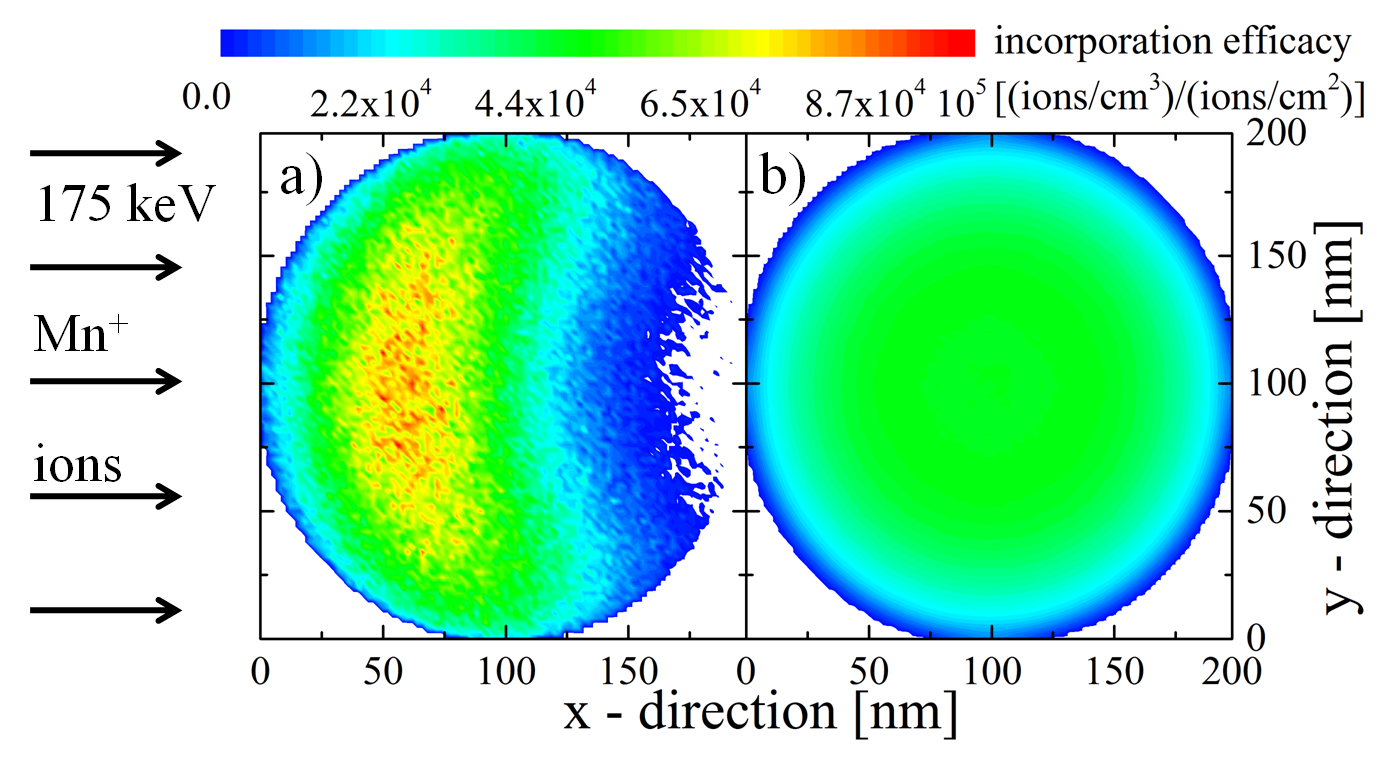
\includegraphics[width=.8\textwidth]{images/iradinacrosssection.png}
	\caption{a) Color plot of the increase in concentration per fluence for the irradiation of a $ZnO$ nanowire with $175\,keV\,Mn^+$ ions at an angle of $45^\circ$ to the $z$-axis. The energy was selected so that the rotation of this profile produces a radially homogeneous dopant distribution, as shown in b). The mean dopant incorporation efficacy is $3.6\cdot10^4\,\nicefrac{(atoms/cm^3)}{(ion/cm^2)}$.}
	\label{iradinacrossection}
\end{figure} 

As lower energy ions have lower ranges, there are fewer paths that cause the ion to leave the nanowire, particularly in the forward direction. Therefore, the first advantage of decreasing the ion energy is that the doping efficacy is larger for lower ion energies, so a lower irradiation fluence is required to achieve doping at a desired level. Furthermore, lower ion energy impacts also produce less damage in the irradiated matrix. Together with an optimal irradiation temperature, the rotated irradiation was utilized to improve the magnetic properties of $Mn^+$ irradiated $GaAs$ nanowires \cite{borschel_new_2011,paschoal_hopping_2012,borschel_ion-solid_2012,kumar_magnetic_2013,paschoal_magnetoresistance_2014}. 


%In figure \ref{iradinacrossection}b the outermost layer of the nanowire has a lower dopant incorporation efficacy than the rest of the wire volume. The sputtered atoms predominantly originate from this outer layer, so that the matrix of the nanowire is eroded preferentially to the incorporated dopants. 

\vfill
\section{nano-XRF on single nanowires}

The expected non-linear increase in doping concentration with the ion fluence was first investigated on $ZnO$ nanowire samples grown in Jena, such as the one shown in figure \ref{ZnOwires}a. The nanowires were transferred onto the carbon-foil of a $Cu$ TEM grid by imprinting after the rotated irradiation with $0.24, 0.48, 0.95$ and $1.9\cdot 10^{17}\,\nicefrac{ions}{cm^2}\,Mn^+$ ions at $175\,keV$; corresponding to $Mn/Zn$ ratios of $0.02, 0.04, 0.08$ and $0.16$, as extrapolated from the mean doping efficacy obtained from the \emph{iradina} simulation.

\begin{figure}[H]
	\centering
		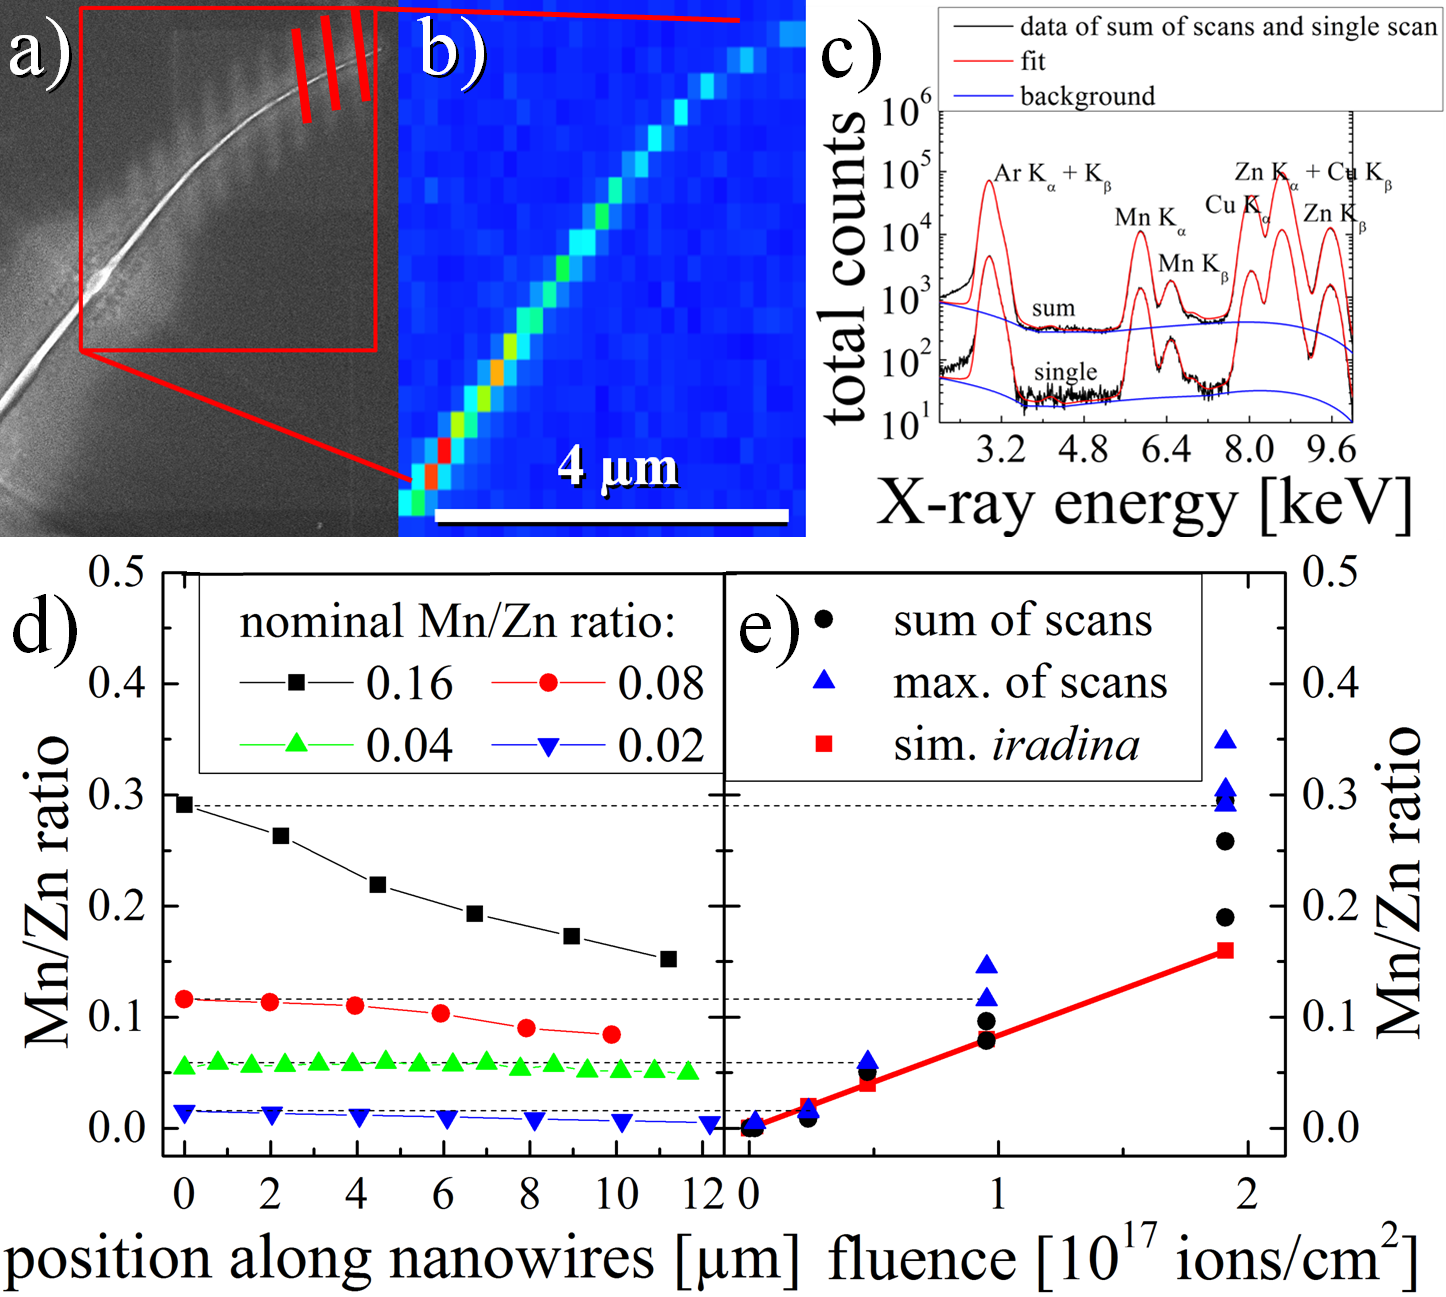
\includegraphics[width=.7\textwidth]{images/largeXRF.png}
	\caption{a) SEM image of a $175\,keV\,Mn^+$ irradiated $ZnO$ nanowire on the carbon-foil of a $Cu$ TEM grid after XRF investigation. The red lines indicate where the focused X-ray beam was scanned with a long integration time. b) Intensity map of the X-ray signal. c) Exemplary XRF-spectra of a single scanned line and for the sum of all the lines for the nanowire shown in a) and b). d) $Mn/Zn$ ratio quantified with PyMCA for representative wires along the length of the nanowires for varying nominal concentrations. The corresponding data points in the plot of the concentration versus the irradiated ion fluence in e) are connected with a dashed line. The red data points and line in e) indicate the linear extrapolation to the nominal $Mn/Zn$ ratio from \emph{iradina} simulations. The black circles show the average ratio obtained by fitting to the sum of all scans, while the blue upturned triangles show the maximum ratio found for along the length of a nanowire.} 
	\label{largeXRF}
\end{figure} 

Figure \ref{largeXRF}a shows a SEM image of one of the $Mn^+$ irradiated $ZnO$ nanowires investigated by nano-XRF at the ESRF. At one point the nanowire shows some damage where the exposure to the XRF-beam was prolonged during the navigation on the sample. Also the track of the intense, focused X-ray beam can be seen on the carbon foil by some redeposition of material. All in all, the damage to the nanowire is, however, not large enough to have an effect on the quantification, especially considering that this particular nanowire was selected as it showed the most pronounced effects. In \ref{largeXRF}b a map of the detected X-ray intensity clearly shows the nanowire. The XRF spectrum collected for one of the scans indicated in the SEM image \ref{largeXRF}a is shown in \ref{largeXRF}c. The number of counts for a single scan is comfortably sufficient to quantify the $Mn$ and $Zn$ content. The average concentration for a nanowire was determined by fitting the sum XRF-spectrum of all scans across the nanowire. The $Mn/Zn$ ratio is plotted over the position along the nanowire for the four nominal concentrations in figure \ref{largeXRF}d. Clearly there is a significant gradient in the $Mn$ concentration along the nanowire length. The maximum $Mn/Zn$ ratio was always found at the tip of the nanowire, which was identifiable in the SEM images by the slight tapering of the nanowires. The $Mn/Zn$ ratio for both the sum of all scans, as well as the scan at the tip showing the maximum $Mn/Zn$ ratio is plotted in \ref{largeXRF}e alongside the nominal ratio extrapolated from \emph{iradina} simulations.
  
Two pieces of information can be gained from these results. First, the nanowires on the sample clearly shadowed each other from the ion beam, leading to the pronounced $Mn$ concentration gradient. The shadowing is least at the tips of the nanowires, therefore the corresponding data points are the closest to the simulated situation. This emphasizes the second point, that the increase in $Mn$ concentration with the ion fluence is much stronger than the linear extrapolation from static simulations. The assumption underlying the doping efficacy gained from the earlier simulations and using it to calculate the required fluence for a desired doping concentration is that the concentration increases linearly with the irradiated fluence. However, this is only true in the absence of sputtering. Sputtering erodes the target nanowire at the same time as ions are incorporated. It thus leads to a non-linear increase in the concentration of dopants with the irradiated fluence. To separate these two effects the irradiation and quantification has to be repeated with nanowires with a sparser lateral distribution, as shown in \ref{ZnOwires}b. These were kindly provided by Dr. Helena Franke from the University Leipzig.

\begin{figure}
	\centering
		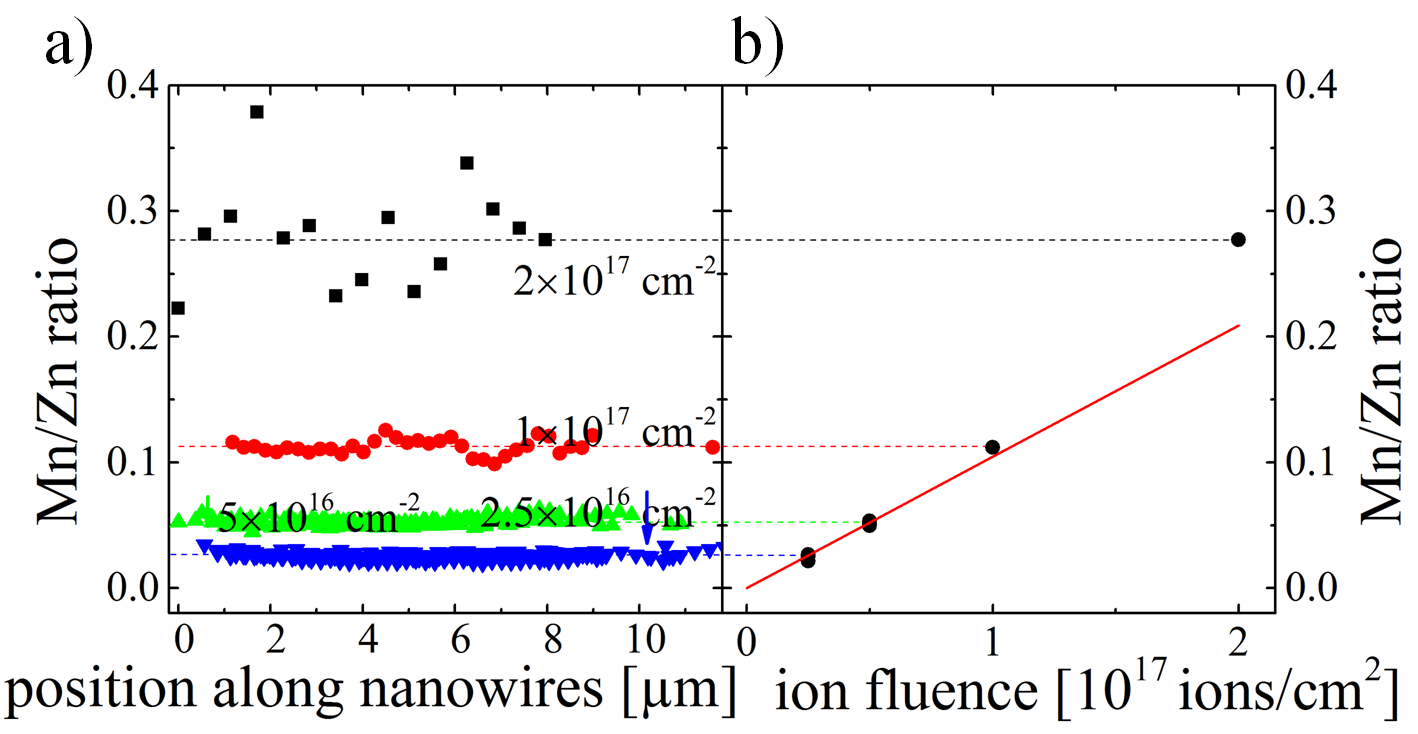
\includegraphics[width=.85\textwidth]{images/MnZn2.png}
	\caption{a) $Mn/Zn$ ratio along the wire length for sparse nanowire samples irradiated with the indicated ion fluence of $175\,keV Mn^+$. There is no concentration profile along the wire length. In b) the black circles show the average ratio obtained by fitting to the sum of all scans for the respective ion fluence. The red line in b) shows the linear extrapolation from \emph{iradina} simulations. }
	\label{MnZn2}
\end{figure} 

The same experimental procedure was followed to investigate the Mn/Zn ratio with the sparser nanowire samples, only rounding the rotated irradiation fluence to $0.25, 0.5, 1$ and $2\cdot 10^{17}\,\nicefrac{ions}{cm^2}\,Mn^+$. The results from the nano-XRF quantification of these nanowires is shown in figure \ref{MnZn2}. The $Mn/Zn$ ratio plotted against the nanowire length in \ref{MnZn2}a no longer shows any gradient. As these wires were individually transferred to the lacy carbon TEM grid, they could be investigated by SEM before and after irradiation. The diameter of the nanowire irradiated with the highest fluence was reduced from $202\,nm$ to $93\,nm$ by sputtering, while the lower fluences produced lower reductions in diameter, as expected. From these diameter reductions the sputter yield can again be calculated, yielding values in the range of 5 - 20. As seen in the dedicated study on sputtering these values have a very large spread. Also the $Mn/Zn$ ratio for the nanowires irradiated with higher fluences shows a significant spread due to the fact that the thinned nanowires have a much smaller volume and thus give a lower XRF signal. Added to this, the thinner wires could only be attached to the lacy carbon loosely, so that they drifted much more during the XRF scans making it impossible to increase the integration time significantly to compensate for the lower signal. Nevertheless, the average $Mn/Zn$ ratio is accurate to within $\pm\,0.01$, as it is based on the sum of all spectra including a sufficiently large number of counts. The average values for all irradiated fluences is plotted in \ref{MnZn2}b against the irradiated fluence. As with the denser nanowire sample, again the increase in the $Mn$ concentration is much larger and non-linear than the simple linear extrapolation from the \emph{iradina} simulation. Now we can be sure that the incorporation is not effected by the shadowing of the nanowires amongst themselves.


\section{Pseudo-dynamic simulation}

The direct simulation of the effect of sputtering on the incorporation of dopants into nanowires requires a dynamic simulation program, which also considers the three dimensional geometry of the target. As such software is not currently openly available, a step-by-step investigation using results from static simulations will be undertaken to discuss the observed interaction between dopant incorporation and sputtering.

\begin{SCfigure}
	\centering
		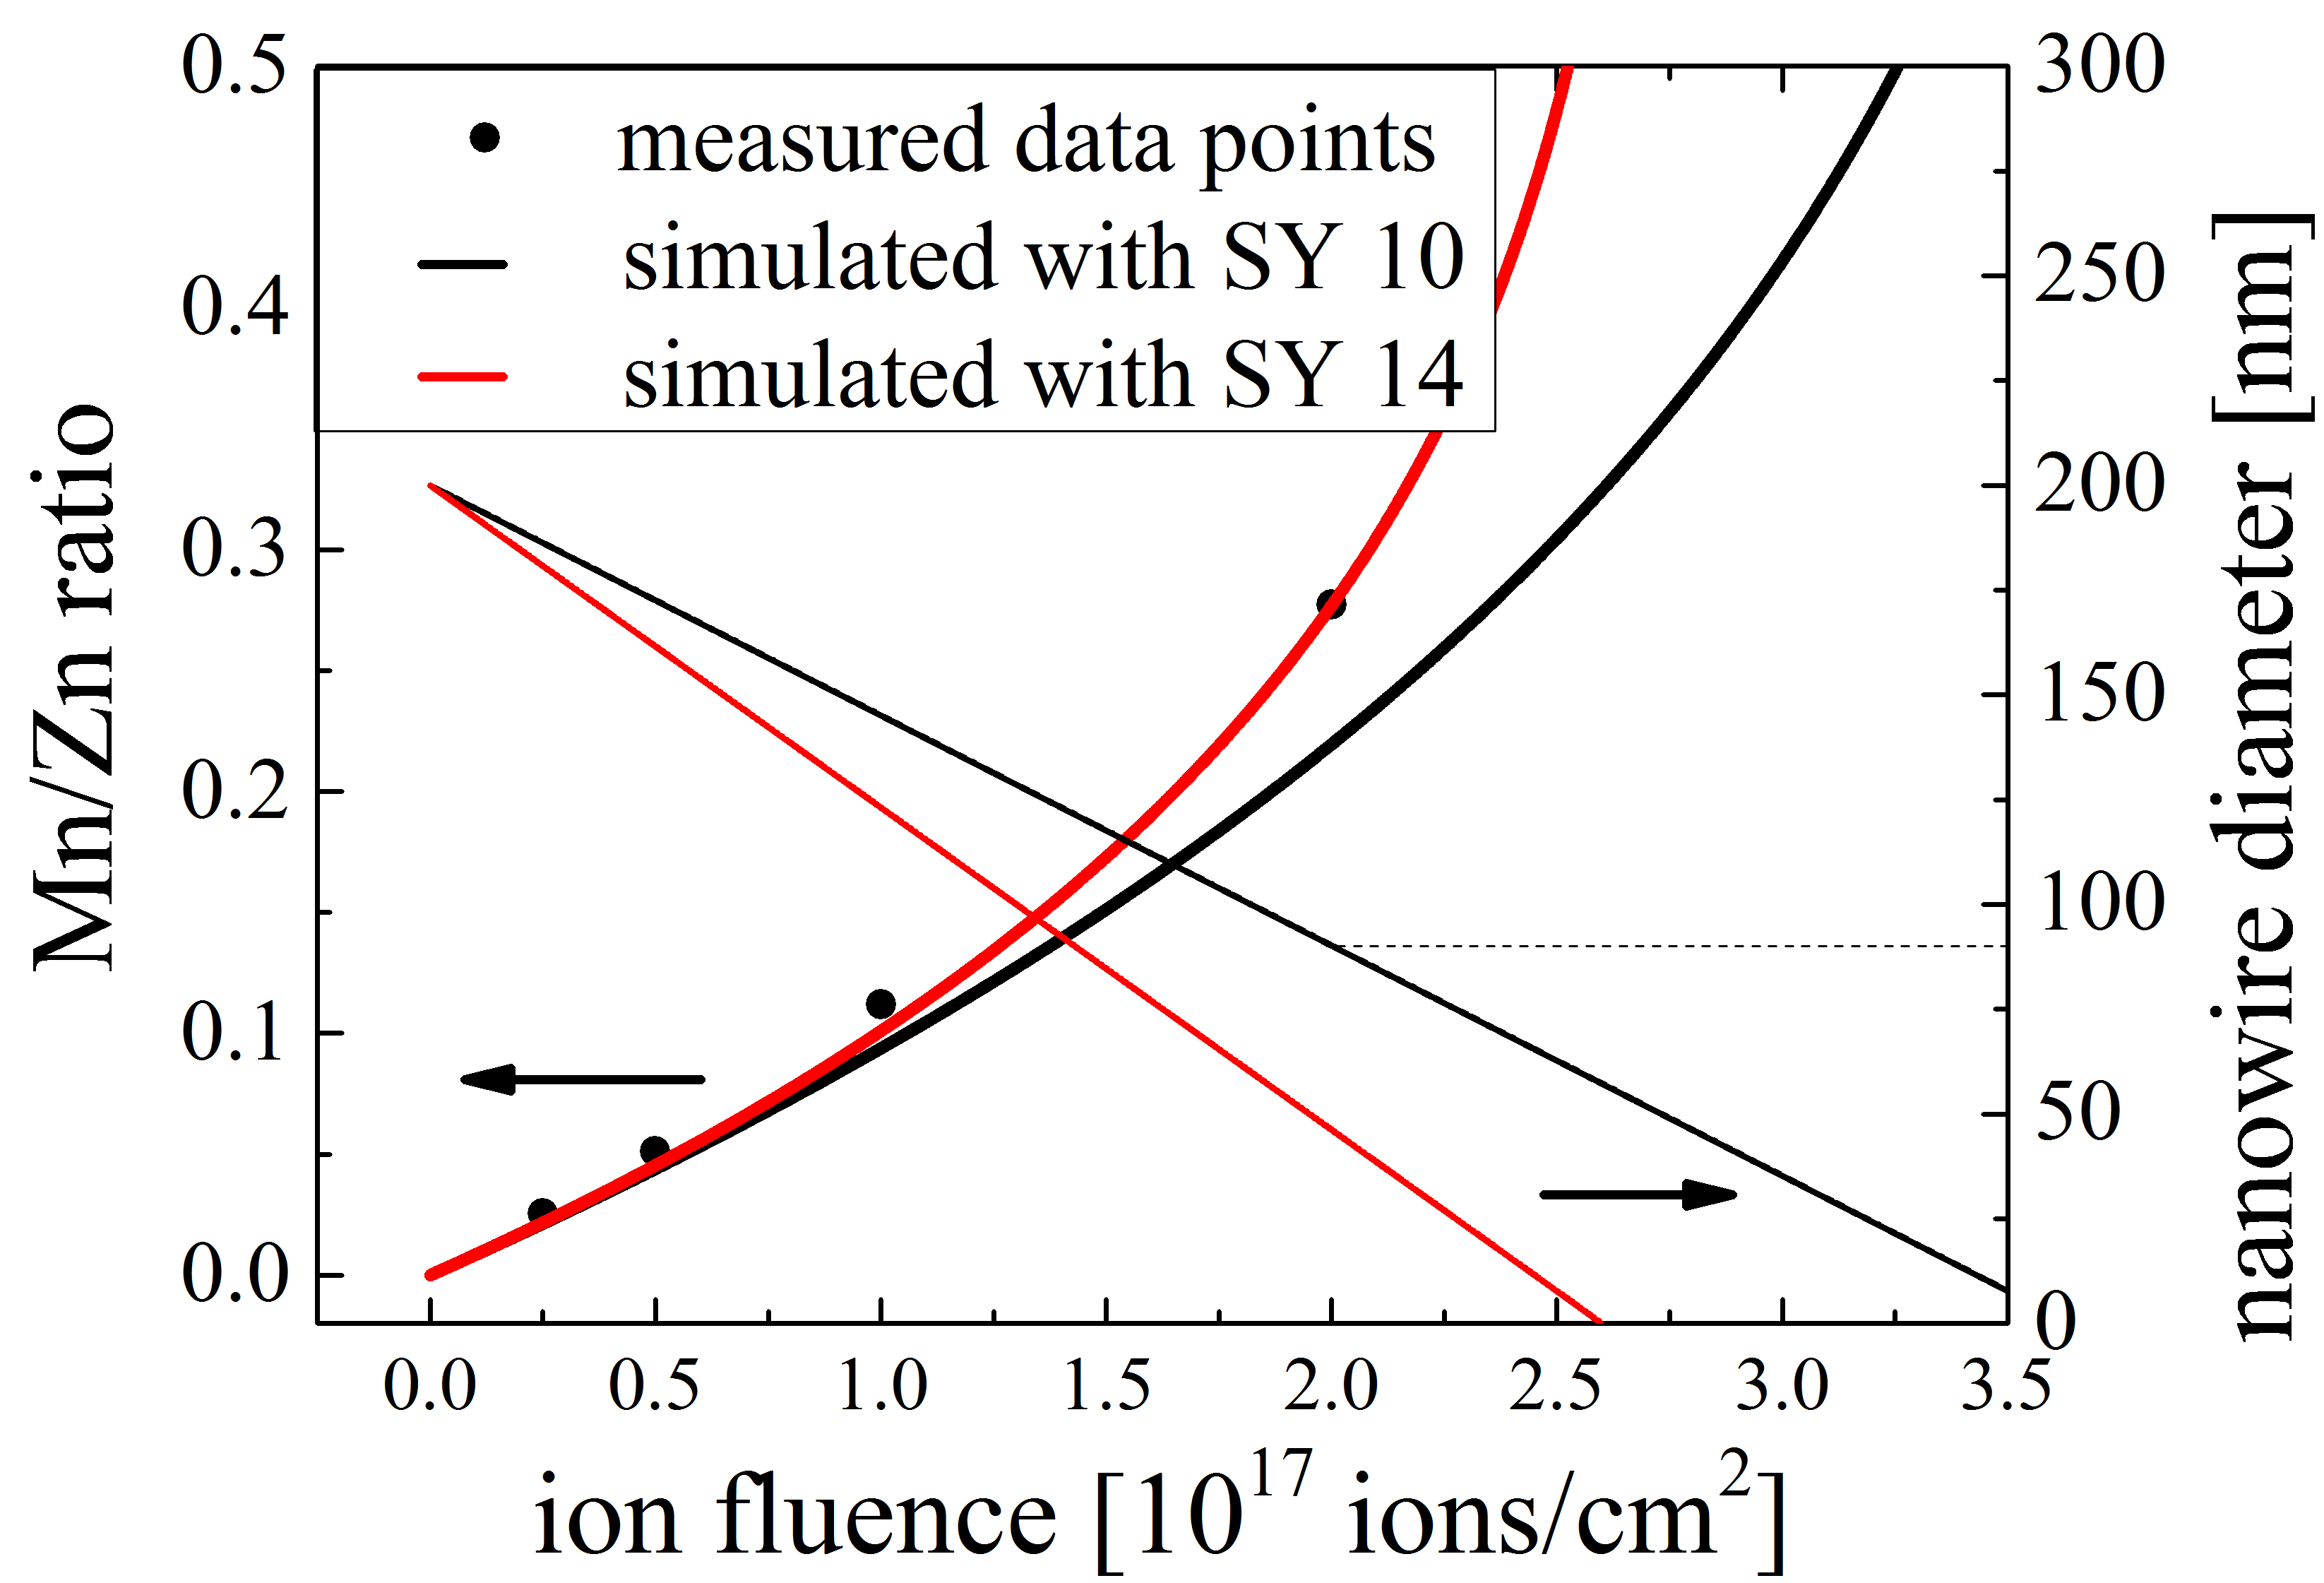
\includegraphics[width=.5\textwidth]{images/staticsputteryield.png}
	\caption{Plot of the $Mn/Zn$ ratio (left axis) versus the irradiated ion fluence of $175\,keV Mn^+$ for the measured nanowires and two simulations, indicated by black circles, a black line and a red line respectively. The nanowire diameter (right axis) is also plotted against the fluence for both simulations. The dashed line at $90\,nm$ marks the final radius of the data point corresponding to the highest irradiated fluence.}
	\label{staticsputter}
\end{SCfigure} 

The most straightforward approach is to consider the total sputter yield and the doping efficacy constant. With these assumptions and a reiterative calculation of incremental fluence steps, a pseudo-dynamic simulation can be numerically constructed. The $Mn$ concentration increases with each irradiated fluence step by the value determined by the doping efficacy. Then the number of $Zn, O$ and $Mn$ atoms is reduced by sputtering so that the total sputter yield is divided between $Zn+O$ and $Mn$ according to the current $Mn$ concentration. The total number of atoms is used to calculate the new nanowire radius and the next incremental fluence step can be calculated. Figure \ref{staticsputter} shows the experimentally determined $Mn/Zn$ ratios next to such a simulation. The doping efficacy was set to the same value used for the linear extrapolation so far, $3.6\cdot10^4\,\nicefrac{(atoms/cm^3)}{(ion/cm^2)}$. The total sputter yield was set to 10 for the simulation yielding the values depicted in black. This value corresponds to the sputter yield determined from the reduction in the radius of the nanowire irradiated with $2\cdot10^{17}\,\nicefrac{ions}{cm^2}$ and therefore, unsurprisingly, this simulation produces the the correct diameter of $\approx\,90\,nm$ at this ion fluence. However the calculated $Mn/Zn$ ratio is too low. Conversely, a simulation with a larger sputter yield of 14, indicated in red, correctly reproduces the $Mn/Zn$ ratio, but erodes the nanowire too quickly. Nevertheless, the overall agreement between the experiment and the simulation seems promising.

To increase the accuracy of the pseudo-dynamic simulation, results from a set of static simulations for varying diameters can be used. The sputter yield is dependent on the nanowire radius and the ion energy as shown in \ref{sputterincorporate}a. This relation is discussed in detail in the previous chapter \ref{sec:simsputering}. Likewise the incorporation efficacy plotted in \ref{sputterincorporate}b is also dependent on the nanowire radius and the ion energy. For a fixed diameter and increasing ion energy the efficacy is monotonically decreasing, as the probability of the ion to leave the nanostructure rises together with the ion range. For fixed ion energies, the probability of an ion to stay in the nanostructure increases with increasing diameter, so that at first the efficacy also increases with increasing diameter. For large diameters this effect is overcompensated by a stronger dilution of the dopants in the volume of the nanowire which increases as the square of the diameter. This leads to a maximum in the incorporation efficacy at diameters around twice the ion range. Note that the color scale in \ref{sputterincorporate}b is logarithmic.

\begin{figure}
	\centering
		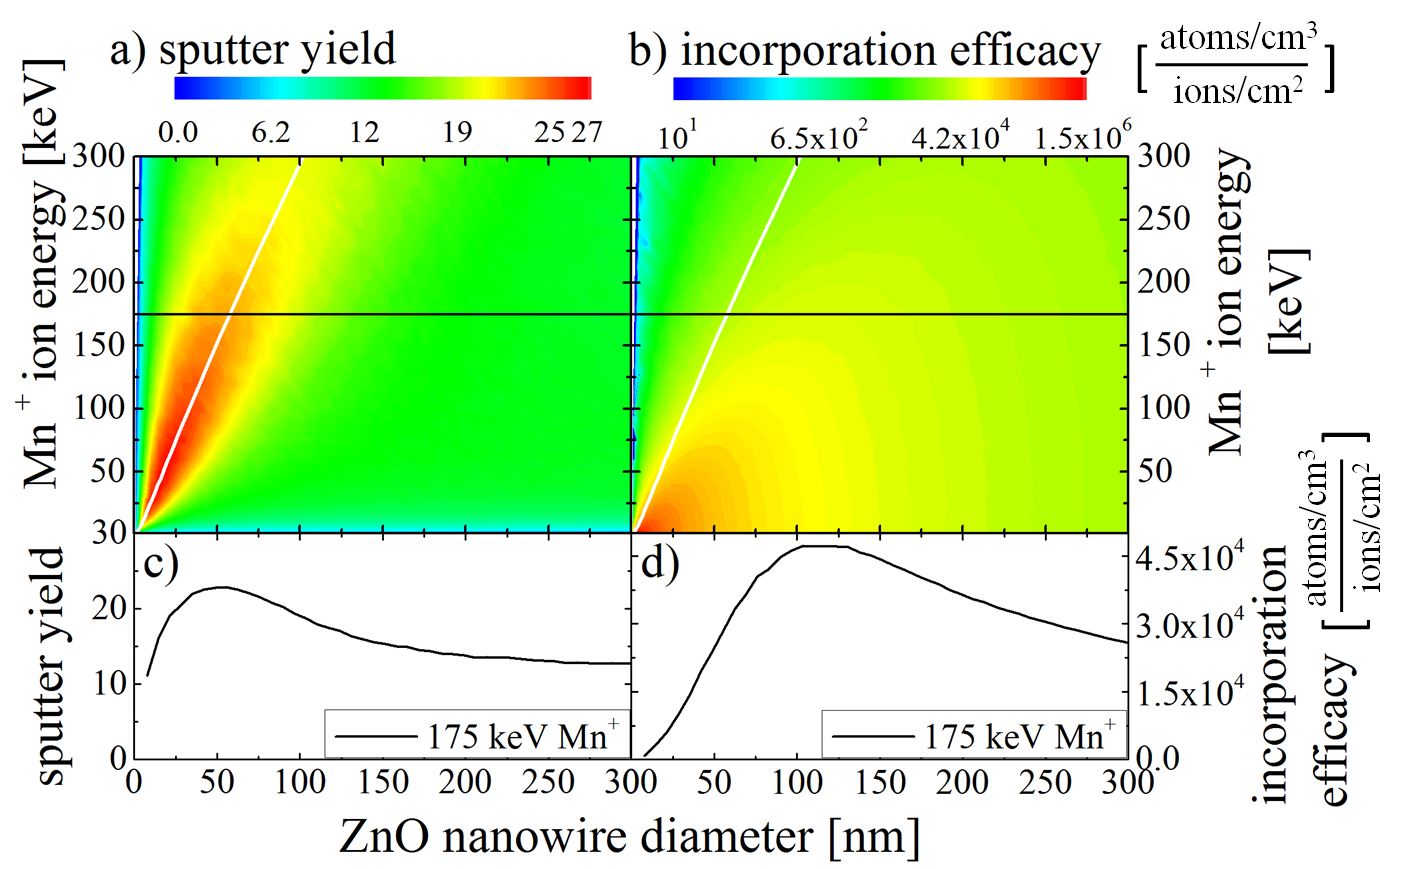
\includegraphics[width=.85\textwidth]{images/sputterincorporate.png}
	\caption{a) Sputter yield for the irradiation with $Mn^+$ of ZnO nanowires with varying diameters an ion energies. From the same simulations the dopant incorporation efficacy was determined and plotted in b). The white line in both plots indicates the ion range at the respective energy and $45^\circ$, calculated with SRIM for $Mn^+$ in $ZnO$. The horizontal black line indicates the energy used in the experiments and simulations in this chapter.}
	\label{sputterincorporate}
\end{figure} 

The numerical, pseudo-dynamic simulation can easily be adapted to use the diameter dependent values for the sputter yield and the dopant incorporation efficacy. The resulting $Mn/Zn$ ratios from such an simulation are plotted in figure \ref{pseudodynamic} as red squares. The stronger than linear increase in the $Mn/Zn$ ratio seems less pronounced in this simulation when compared to the simulation only considering constant sputtering and doping efficacy, as the doping efficacy starts decreasing markedly with decreasing diameter from diameters around $100\,nm$. Here, also the sputtering starts to increase as the ions start to reach the back of the now thinned nanowire. In the evolution of the diameter with the irradiated ion fluence, plotted in figure \ref{pseudodynamic} as a red line, the increased sputtering is noticeable as a slight increase in the slope of the curve at $2\cdot 10^{17}\,\nicefrac{ions}{cm^2}$.

\begin{SCfigure}[50][h]
	\centering
		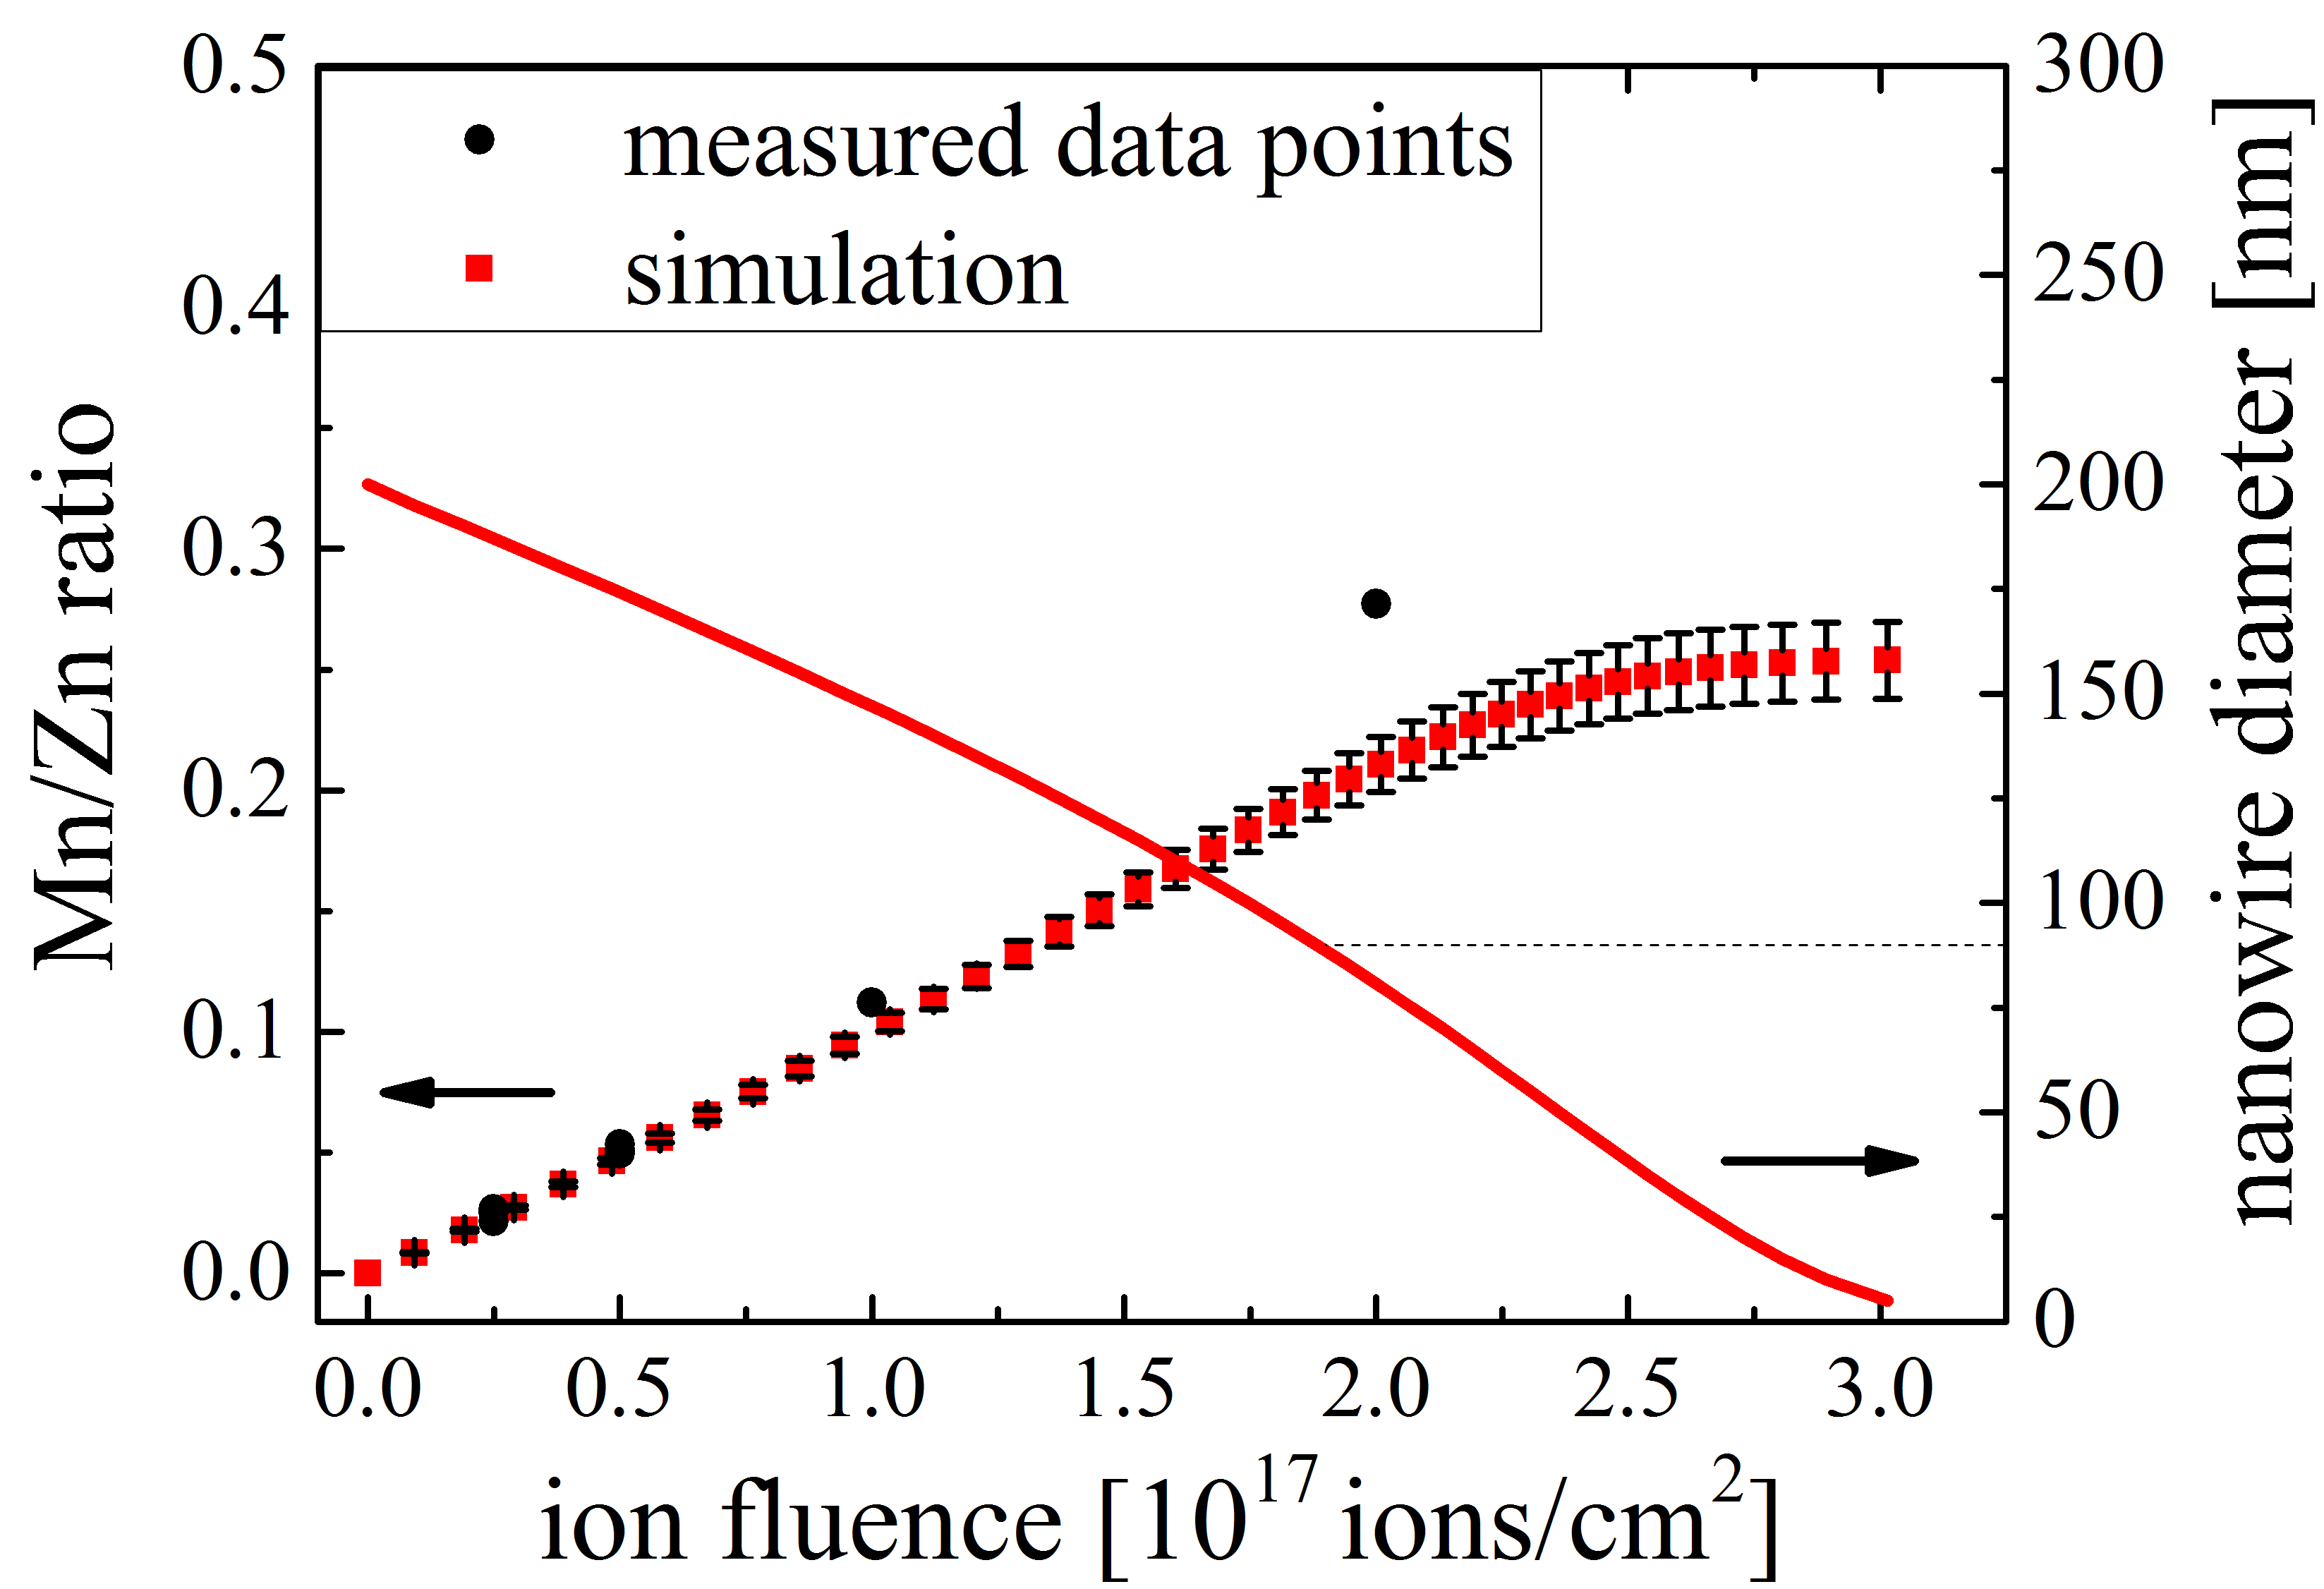
\includegraphics[width=.5\textwidth]{images/pseudodynamic.png}
	\caption{Results from a pseudo-dynamic simulation considering diameter dependent sputtering and doping efficacy. The $Mn/Zn$ ratio is plotted to the left axis versus the ion fluence of $175\,keV Mn^+$ as red squares for the simulation and black circles for the experiment. The error bars range from the $Mn/Zn$ ratio for $170\,keV$ to $180\,keV Mn^+$. The red line indicates the simulated nanowire diameter.}
	\label{pseudodynamic}
\end{SCfigure} 

\section{Discussion of relevant effects}

\subsubsection{Summarizing Discussion}

%\chapter{Plastic Flow in Silicon Nanowires}

\section{Discovery}

Within the ``wiring quantum dots'' project $Si$ nanowires where irradiated with $As^+$ and $In^+$ and/or $Ga^+$ so that in a subsequent annealing step $Si-GaAs$ or $Si-InGaAs$ hetero-structures could be formed. Markus Glaser, the Ph.D. student responsible for this part of the project, had developed a good habit of making SEM images of the same individual wires after each process step. We thus noticed, that the $Si$ nanowires shrank quite dramatically during the irradiation with $\approx 100\,keV$ $In^+$, $Ga^+$ and $As^+$ at room temperature. Two examples of this can be seen in figure \ref{deformSEM}. A look into literature revealed that this behavior has so far not been reported for irradiation of $Si$ at such low ion energies. A thorough investigation might be worthwhile. 
 
\begin{SCfigure}
	\centering
		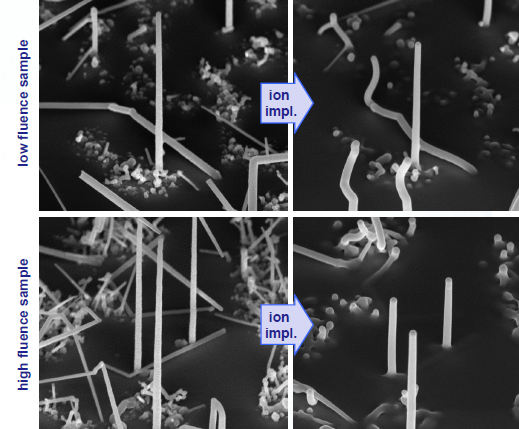
\includegraphics[width=.48\textwidth]{images/deformSEM.png}
	\caption{\textcolor{red}{placeholdergraph - get nicer image from Markus.} SEM images of VLS-grown $Si$-nanowires before and after the irradiation with X In and Y As at room temperature, while rotating the sample. The shrinking and widening of the wires is clearly visible. In the background wires which were not aligned perpendicular to the substrate are bent upward.} 
	\label{deformSEM}
\end{SCfigure}

Similar $Si$ nanowire arrays as the ones used for the sputtering experiment were thus systematically irradiated with $Ar^+$, making SEM images after each irradiated fluence to observe and quantify the deformation. $Ar$ was chosen for the irradiation to avoid any chemical effects and because it has a comparable mass to $Ga$ and $As$. Using the algorithm described in the sputter yield chapter, the profiles for the irradiated nanowires could be extracted. In figure \ref{deformationprofile} the black, red, green and blue lines indicate the height dependent diameter of a single wire before and after irradiation with $100\,keV\,\,Ar^+$ up to fluences of 1, 3 and $5 \times 10^{16}\,cm^{-2}$ respectively. In this graph, as well as in the inset black profiles, the reduction of the height by $\approx 500\,nm$ and an increase of the diameter, especially at the base, can be clearly seen. The deformation is only seen with irradiation at room-temperature where $Si$ amorphization threshold of $10^{14}\,ions/cm^2$ for $100\,keV\,\,Ar^+$ is very low \cite{pelaz_ion-beam-induced_2004}.

\begin{SCfigure}
	\centering
		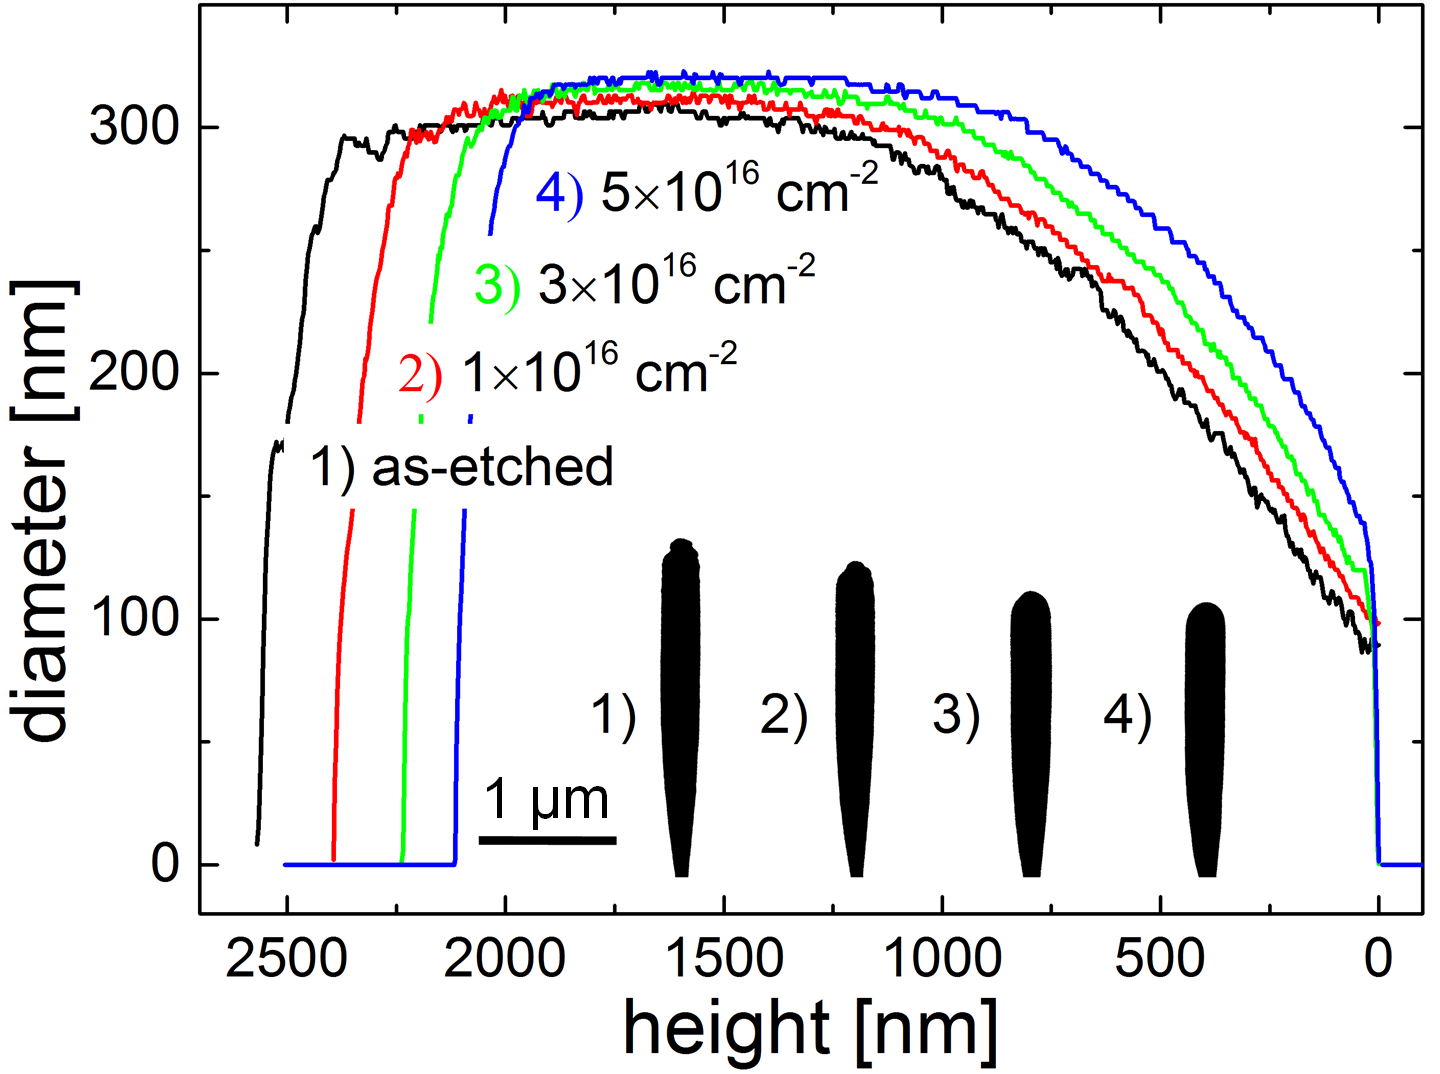
\includegraphics[width=.48\textwidth]{images/deformationprofile.jpg}
	\caption{Graphs of the diameter over height of a single $Si$ nanowire irradiated with increasing fluences of $100\,keV Ar^+$ ions. The black insets show the profiles of the nanowire after the respective fluences extracted from SEM images. In both illustrations the shrinking and widening of the wire is clearly visible.} 
	\label{deformationprofile}
\end{SCfigure}

\section{Quantification}

The deformation of the nanowires can be roughly quantified by fitting a linear trend to the fluence dependence of the height of the wires. This yields an average of $3\%$ shrinkage per $10^{16}\,ions/cm^2$. Due to outliers with larger deformation the values obtained for the 21 nanowires investigated have a large standard deviation of $\pm 3\%$ shrinking per $10^{16}\,ions/cm^2$. A more thorough investigation of the deformation is possible by also accounting for the height dependence of the diameter seen in figure \ref{deformationprofile}. On average a certain number of atoms are displaced by a certain distance along the height $z$ of the nanowire per ion. Considering only the movement along the height $z$, a mass-transport rate (MTR) can be calculated according to equation \ref{MRTequation}:

\begin{equation}  
\begin{split}
    MTR_{(1 \rightarrow 2)} & = [ {}^{1}N\cdot {}^{1}z_{c} -{}^{2}z_{c} \cdot {}^{2}N - ({}^{1}N - {}^{2}N) \cdot {}^{2}z_{c}]/N_{ion} \\
		& = {}^{1}N \cdot ({}^{1}z_{c} - {}^{2}z_{c})/N_{ion} 
	\label{MRTequation}
	\end{split}
\end{equation}

\begin{SCfigure}[50][h]
	\centering
		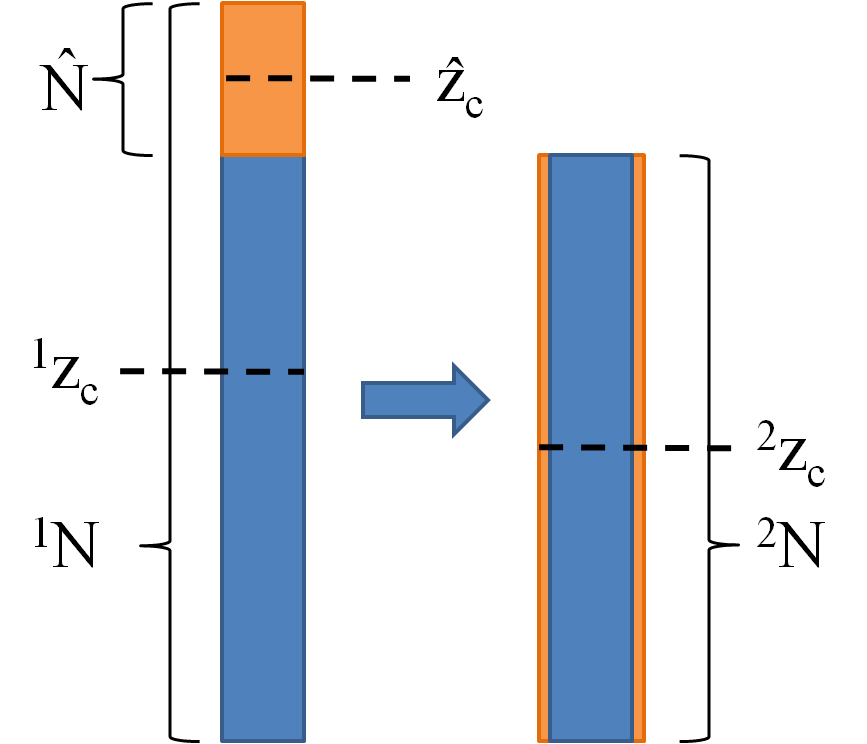
\includegraphics[width=.25\textwidth]{images/MTRillustration.png}
	\caption{Illustration of the mass-transport rate calculation. Displacing ${}^{1}N$ atoms from their average height ${}^{1}z_{c}$ to the average height ${}^{2}z_{c}$ requires the same mass-transport, as moving $\hat{N}$ from $\hat{z}_c$ to ${}^{2}z_{c}$, taking into account the sputtered atoms ${}^{1}N-{}^{2}N$.}
	\label{MTRillustration}
\end{SCfigure}

In equation \ref{MRTequation} and figure \ref{MTRillustration}, ${}^{1/2}z_{c}$ is the height of the center of mass of the nanowire with the top left index indicating before ($^1$) and after ($^2$) irradiation respectively. The number of atoms at height $z_i$ can be calculated from the local radius $r_i$. Summing up the height weighted by the number of atoms at that height $z_{c} \cdot N = \sum_i{\pi r_i^2 h \cdot \rho \cdot z_i}$ and dividing this by the total number of atoms $N = \sum_i{\pi r_i^2 h \cdot \rho}$ in the nanowire gives us $z_{c}$. The sums are over all slices $i$ of height $h = 1\,pixel = 2.7\,nm$ (typically) each. The number of ions that hit the nanowire in the irradiation of fluence $\Phi_{12}$ between making SEM images $1$ and $2$ is $N_{ion} = \sum_i{({}^{1}r_i+{}^{2}r_i)}$ $\cdot sin(45^\circ) \cdot h \cdot \Phi_{12}$. The last term in equation \ref{MRTequation} accounts for the influence of sputtered atoms. Just as in the chapter on sputtering, the sputter yield could be calculated by $({}^{1}N - {}^{2}N)/N_{ion}$. Figure \ref{MTRillustration} illustrates two interpretations of the MTR calculation. As only the displacement along $z$ is considered, the direct interpretation of equation \ref{MRTequation} of moving ${}^{1}N$ atoms from their center of gravity ${}^{1}z_{c}$ to a new center of gravity ${}^{2}z_{c}$ is equivalent to moving the atoms which are `missing' at the top of the wire after the irradiation ($\hat{N}$, orange volume in figure \ref{MTRillustration}) from their center of gravity $\hat{z}$ to ${}^{2}z_{c}$, and subtracting the sputtered atoms. This evaluation yields an average mass-transport rate of $1.2\cdot10^4 \,atoms \cdot  nm / ion$ with a standard deviation of $7\cdot 10^3\,atoms \cdot nm / ion$. Again the large standard deviation is due to outliers with larger deformation.

\section{Knock-on transport of mass}

A possible explanation for this behavior can be sought in the linear cascade theory which is applicable for the cascades of $100\,keV\,\,Ar^+$ in $Si$. In a collision cascade following an energetic ion impinging a solid, atoms will be preferentially `knocked-on' along the propagation direction of the impinging ion. This causes an inhomogeneous distribution of interstitials and vacancies and effectively mass is transported `downstream' along the ion beam. In an amorphous material it is not clear what constitutes an `interstitial' or a `vacancy', but a local excess of vacancies can be understood as a locally decreased density, while an interstitial excess corresponds to an increased density. A local density gradient is not stable, since the density of amorphous $Si$ before and after irradiation is not significantly different \cite{pelaz_ion-beam-induced_2004}. Therefore, the density gradient introduces stress in the material which can relax by plastic deformation, possibly enabled by a decreased viscosity due to further ion irradiation \cite{snoeks_stress_1997,hu_burrowing_2002,mayr_mechanisms_2003,mayr_effect_2003}. 

As was shown in the example of sputtering, BCA simulation software can accurately reproduce linear collision cascades. Therefore, comparing the experiments with a simulation with \emph{iradina} can evaluate whether the deformation observed in the experiment can be accounted for by knock-on mass transport. Figure \ref{deformationBCA}a shows the simulation volume implemented in \emph{iradina} with $2\times2\times2\,nm^3$ voxels as a $600\,nm$ long $Si$ cylinder with a diameter of $200\,nm$. The $100\,keV\,\,Ar^+$ ions impinge at an angle of $45^\circ$ to the $z$-axis. They strike the cylinder distributed uniformly along the $y$-direction at height $z=0$. Figure \ref{deformationBCA}d shows the resulting distribution of interstitials on the cross-sectional slice through the middle of the nanowire along the $xz$ plane. This can be seen as an approximation for the distribution of the nuclear energy loss and shows the mean extent of the collision cascade. Figure \ref{deformationBCA}e shows the same cross-section after subtracting the number of vacancies produced per ion from the number of interstitials. The excess of vacancies along the impinging plane (blue cone in the cross section) enveloped by two red planes of excess interstitials shows that there is a high probability for the ions to hit a target atom with a large impact parameter. This changes the ions path only little and displaces the target atom in an direction perpendicular to the ion beam. Superimposing many collisions along the $y$ direction leads to the formation of one one vacancy rich and two interstitial rich planes. The $xy$-plane in \ref{deformationBCA}b shows the sum over the height $z$ of the difference between interstitials and vacancies plotted to the same color scale. The illustration is dominated by vacancies at the surface of the cylinder which are left behind by sputtered atoms. 

The height distribution (summing over the radial $xy$ plane) of the interstitials, vacancies and leaving atoms is shown in \ref{deformationBCA}c. As expected, the majority of sputtered atoms originate near the impact height. The lines showing the interstitials and vacancies overlap in this illustration. The vacancies subtracted from the sum of interstitials and leaving atoms is plotted along the height in \ref{deformationBCA}f. As a displaced atom, leaving behind a vacancy, is either sputtered or becomes an interstitial, the sum over all heights of of this graph is zero. The strong oscillation around $z=0$ in \ref{deformationBCA}f is caused by the previously discussed displacement of target atoms at an angle almost perpendicular to the ion beam for large impact parameters. This oscillation is very sensitive to the voxel-size as in effect the voxel size defines a recombination length and interstitial and vacancy rich regions are mixed in larger voxels. On the other hand, the excess of vacancies near the impact point ($\le 70\,nm$) and of interstitials further down along the ion's path ($\approx 100\,nm$) is not sensitive to the voxel size. It can be used to quantify the knock-on mass transport by multiplying the plotted values by their height and integrating over all heights. The influence of the short range oscillation immediately around the impact point disappears as here $z \approx 0$ is small. The value obtained from this calculation is $78\pm1\,atoms \cdot nm /ion$. Clearly this value is to low to account for the large deformation observed in the experiment where a mass-transport rate of $\ge 1\times 10^{4}\,atoms \cdot nm /ion$ was assessed.

\clearpage
\begin{figure}[thbp]
	\centering
		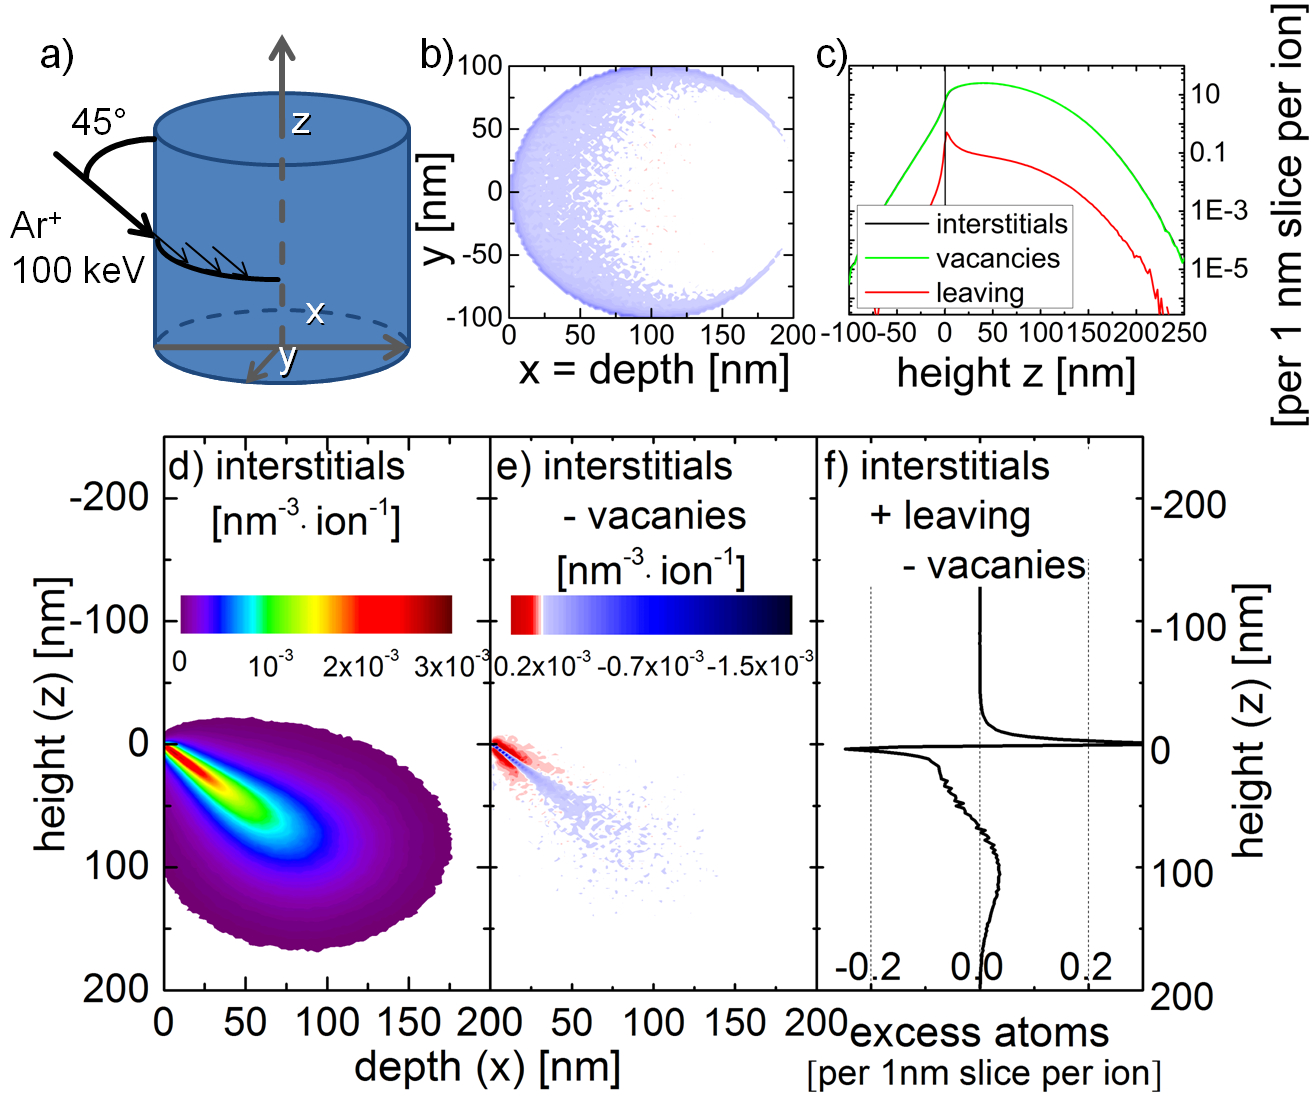
\includegraphics[width=8cm]{images/deformationBCA.jpg}
		\caption{a) Illustration of the simulated irradiation geometry. All $Ar^+$ ions of $100\,keV$ energy hit the nanowire volume at the same height and at an angle of $45^\circ$ with respect to the wire axis $z$. The created interstitials in the radial cross-section through the middle of the simulated nanowire is shown in d). This distribution is effectively an illustration of the nuclear energy loss. In e) the vacancies are subtracted from the interstitials for the same cross-section. Summing this difference over all heights gives the radial distribution shown in b). The clear dominance of vacancies near the surface is caused by sputtering. The axial profile of the interstitials, vacancies and leaving (sputtered) atoms plotted in c) over the height relative to the impact plane shows that most atoms are sputtered at the impact height. Note that the plots of vacancies and interstitials overlap. The vacancies subtracted from the sum of interstitials and sputtered atoms plotted over the height in f) shows mass transport along the ion's path. Apart from the strong oscillation at the impact height, there is a deficiency of atoms close to the impact height ($\le 70\,nm$) and an excess centered around $100\,nm$ down from the impact height.} 
	\label{deformationBCA}	
\end{figure}

As a little excursion, it has to be noted that BCA software typically checks at each collision whether the target atom acquires more energy than the ``displacement energy'' which is a material specific parameter. If an atom has less than the displacement energy after a collision, it is assumed to remain bound in its place and the energy is converted into lattice vibrations ($=$ heat). The displacement energy is experimentally accessible for crystalline materials by electron irradiation experiments in which the irradiating electron energy is in the order of $MeV$. From the electrons' impulse and mass the maximum transferred energy can be calculated. The defects produced as a function of electron energy can thus be used to determine a threshold energy for point defects. This value is defined as the displacement energy. For all simulations a reasonable value for crystalline $Si$, $15\,eV$ \cite{corbett_production_1965}, was used. It is questionable what this value is supposed to mean, as point defects are not well defined in an amorphous medium. Therefore, simulations where repeated with the displacement energy set to $0\,eV$. As expected, the number of `vacancies' and `interstitials' now produced by the simulation increased dramatically. However, the long range difference between `vacancies' and `interstitials' is unchanged. This is an indication that the knock-on mass transport is dominated by the rare events where target atoms are hit directly by the impinging ions. In these cases, a large amount of energy is transferred to the displaced atom leading to a long trajectory within the material. The atoms displaced with lower energies are much more numerous, but travel much shorter distances and in a randomly orientated direction. This is because most of the low energy displaced atoms are generated at the end of a branch of the collision cascade, the orientation of the branch having previously been randomized by higher energy collisions. And/or they originate from collisions with a high impact factor, which lead to a large angle between the incoming particle's and the displaced particle's momentum, as seen in the separation of interstitials and vacancies near the impact point in figure \ref{deformationBCA}e.

\section{Irradiation at large angles of incidence}

If knock-on mass-transport is not the main contribution to the deformation, the question arises whether the direction of the deformation is related to the ion beam. Will an irradiation from `below the substrate' towards an unconstrained end of the nanowire would also shrink the wire, or stretch it out? Nanowires attached to a substrate are obviously not suited to testing this, so a method to irradiate nanowires while rotating them at angles greater than $90^\circ$ to the ion beam was devised. This was achieved by attaching a $Si$ nanowire grown epitaxially on a $Si$ wafer to an $Au$ microwire which can suspend the nanowire at arbitrary angles in the irradiation chamber. The process is shown in figure \ref{reverseFIB}. The $Pt$ deposition was used to glue the nanowire to the micro-manipulator in the FIB and cut the nanowire from the substrate with the $Ga$-FIB. Using the $Pt$-deposition and $Ga$-FIB again, the nanowire is subsequently attached to the tip of a sharpened $Au$-microwire which was previously glued to a piece of wafer for handling and also placed in the FIB chamber. VLS-grown nanowires were used for this experiment as they were readily available in longer lengths ($>10\mu m$) than the etched nanowires.

\begin{figure}[thbp]
	\centering
		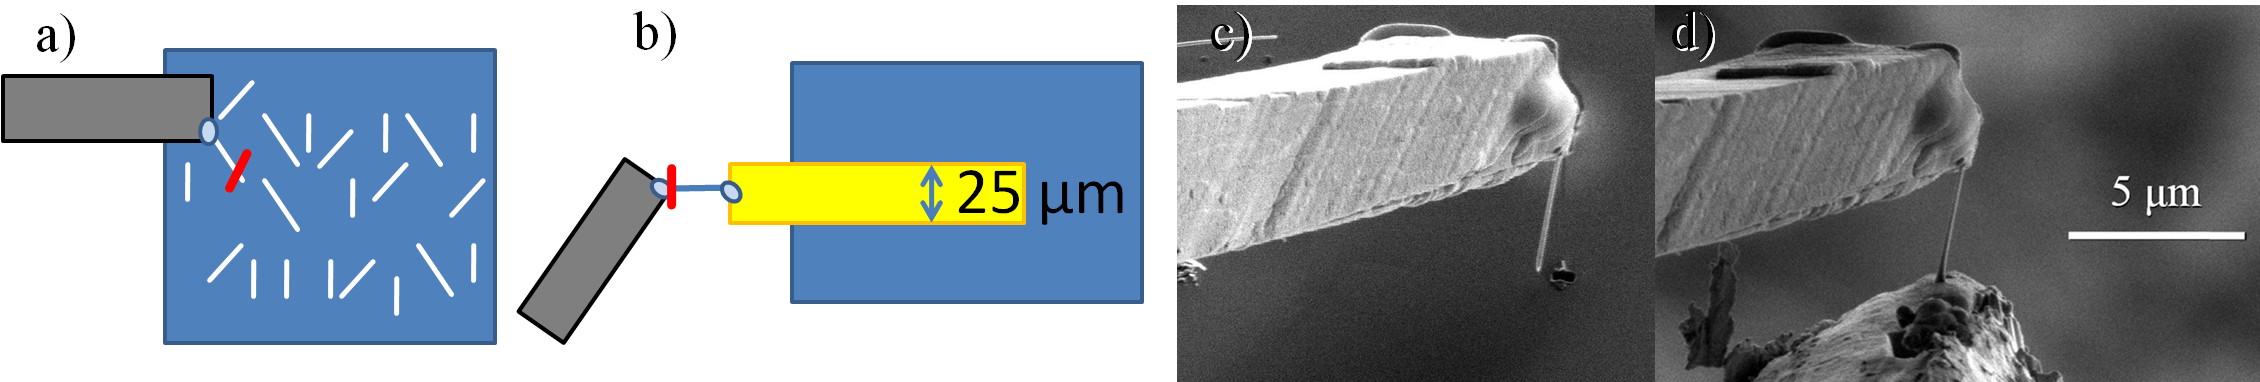
\includegraphics[width=0.99\textwidth]{images/reverseFIB.jpg}
	\caption{Illustration of the nanowire-on-microwire fabrication in a FIB system. The schematic a) and SEM image c) show the wire first glued to the micro-manipulator in the FIB by $Pt$-deposition (light blue ellipse), then cut from the substrate with the $Ga$-FIB (red line). Images b) and d) Illustrate the subsequent gluing to an $Au$ microwire with $Pt$-deposition and the final cut with the $Ga$-FIB to release the nanowire from the micro-manipulator.}
	\label{reverseFIB}
\end{figure}

The nanowire-on-microwire samples consisted of typically $3-5$ nanowires, each attached to an $Au$-microwire and arranged in the irradiation chamber on a rotatable stage at an angle of $135^\circ$ to the ion beam, as shown in figure \ref{reverseangle}a. The alignment of the nanowires to their microwire support was found to be crucial, as any shadowing of a nanowire from the ion beam an one side would lead to extreme bending of the wire. Only a single wire was found straight enough to evaluate quantitatively for more than on irradiation step. The SEM images of this wire are shown in figure \ref{reverseangle}b-f view from a perspective perpendicular to the axis of rotation and rotated by the indicated angle around this axis. The left SEM images show the uniradiated nanowire, while the center and right images were made after the irradiation of $1\times10^{16}\,cm^{-2}$ and $3\times10^{16}\,cm^{-2}$ $100\,keV\,\,Ar^+$, respectively. The uniradiated wire is straight and $3.9\,\mu m$ long. The irradiated wire shows some bending, so the length had to be determined from a perspective were the curvature of the wire is in plane with the image. A fifth order polynomial was fitted to the bent shape and the length of the wire was thus determined to be $3.5\,\mu m$ after $1\times10^{16}\,cm^{-2}$ (\ref{reverseangle}b) and $3.2\,\mu m$ after $3\times10^{16}\,cm^{-2}$ (\ref{reverseangle}f). The nanowire thus shrank with a similar deformation rate to the previously reported $3\%$ strain per $10^{16}\,ions/cm^2$, even though the irradiation was directed towards its free end.

\begin{figure}[thbp]
	\centering
		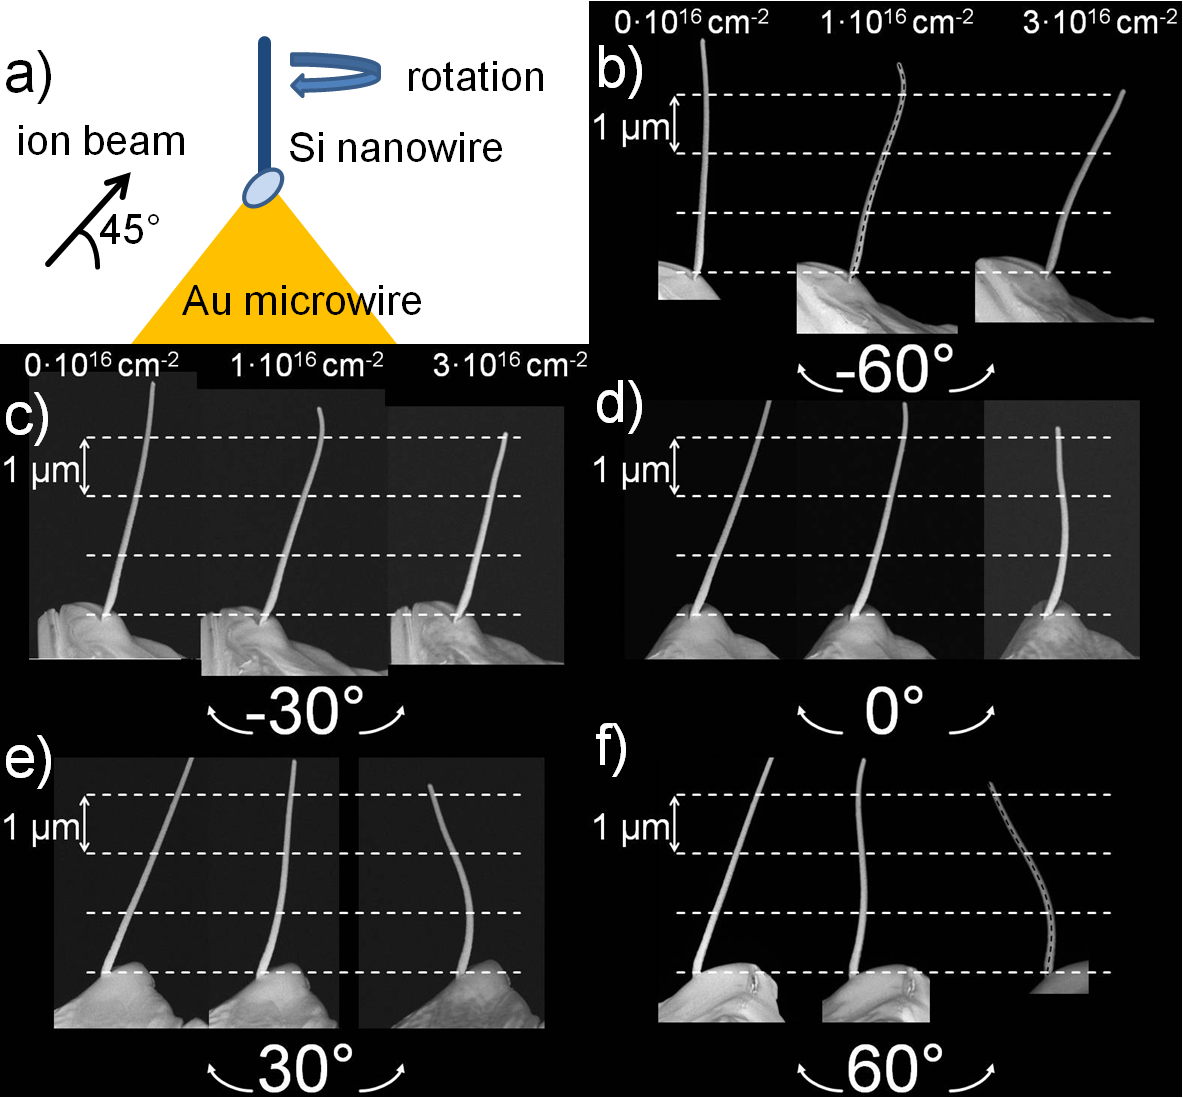
\includegraphics[width=8cm]{images/reverseangle.jpg}
	\caption{ a) Illustration of the nanowire-on-microwire irradiation setup. b) - f) SEM images of the same nanowire as-mounted (left SEM images), after irradiation with $1\times10^{16}\,cm^{-2}$  (center images), and $3\times10^{16}\,cm^{-2}$ (right images) $\,100\,keV Ar^+$ ions. The SEM images where taken with the nanowire rotated by the indicated angle from a perspective perpendicular to the angle of rotation. The length of the nanowire after irradiation is determined in b) and f) along the dashed lines.}
	\label{reverseangle}
\end{figure}

This experiment shows with certainty that the knock-on mass-transport is not the main contributor to the observed deformation, as it would have to be directed along the ion beam. The discussion of a possible model for the deformation will be easier by addressing similar effects and the way that simulation tools were used to understand them. The BCA MC simulation tools available inherently neglect all collective movement of atoms within the target. As has been shown in the previous two chapters, this may be sufficient for the prediction of sputtering and the ion distribution in nanostructures. A field of study which has already faced the limitation of neglecting the local temperature in ion irradiation is the irradiation with swift, heavy ions. At energies well beyond $MeV$ the assumption that the dominating effects will be described by binary collisions between the ion and target atoms is false. At these high energies and ion masses a significant amount of energy will be transferred form the ion to the electronic system of the target. Through the relaxation mechanisms of the electronic system a part of this energy will be converted to heat in the lattice. Under certain conditions this will form ``ion-tracks'' in the target. One approach to understanding the formation and behavior of ion-tracks is to simulate the longitudinal distribution of the deposited ion energy in the target with BCA tools (typically SRIM) and to evaluate the local temperature in a second step by following the deposited energy according to thermodynamic considerations. A good review of such ``thermal spikes'' can be found in \cite{wesch_effect_2004}. 

Such a thermal spike approach was successful at understanding the plastic deformation by swift heavy ion irradiation according to Trinkaus and Ryazanov \cite{trinkaus_viscoelastic_1995} and in the understanding of material properties governing the direction of the deformation \cite{hedler_amorphous_2004,hedler_boundary_2005}. When nanoparticles are deformed \cite{snoeks_colloidal_2000,snoeks_colloidal_2001,van_dillen_anisotropic_2001,dillen_energy-dependent_2001,dillen_ion_2003,dillen_ion_2004} an adapted version of the model by Trinkaus can be applied and the effect dubbed ``ion hammering'' \cite{klaumunzer_ion_2004}. In short, according to this model the local temperature leads to a transient `liquid' phase in the cylindrical volume of material around the ion's path. Within the cylindrical geometry, the deformation by thermal expansion is anisotropic and because stresses can relax in the low viscosity volume, this is a plastic deformation. This is not observed in materials which remain crystalline during the irradiation, as the long range order of the crystal lattice is reinforced upon the recrystallization during cooling. The problem with directly applying this model to the situation at hand is that the total energy density in the collision cascade of $100\,keV\,Ar^+$ in $Si$ is a low $\frac{dE}{dx} = 36\,\frac{eV}{nm}$, of which the electronic energy loss is roughly half. Also, the lowest ion energy for which plastic deformation of silica nanoparticles is reported is $300\,keV Xe^+$ \cite{dillen_ion_2003}. Here the energy loss is merely $\frac{dE}{dx} = 120\,\frac{eV}{nm}$ with $20\,\%$ lost to the electronic system. The threshold for ion tracks, however, is given at $\frac{dE}{dx} \geq 1\,\frac{keV}{nm}$ by Trinkaus et al. \cite{trinkaus_viscoelastic_1995}!

The alternative to thermodynamic considerations after a MC BCA simulation are full MD simulations, where the trajectory and interaction of every atom or ion in the simulation volume is followed. This naturally includes all thermal effects, but is limited by computing power to a low number of atoms and thus a severely limited volume of material. Additionally the accuracy of results depends greatly on finding the interaction potential for all combinations of ions and atoms involved. Here again, as for sputtering, this is true especially for low energy interactions, where these potentials are not available but a topic of research in themselves \cite{primetzhofer_inelastic_2012,primetzhofer_local_2013}. Investigations of the self-irradiation of $10\,keV\,Si$ and various metals \cite{nordlund_defect_1998} revealed the formation of nanoscale `liquid' pockets. The term ``liquid'' must be used with care as it refers to a thermodynamical state of matter while the simulation timescale does not allow the assumption of thermodynamic equilibrium. Nevertheless, a sufficiently large number of atoms gain much kinetic energy (say `are hot') to make the assumption of reduced viscosity and other effects safe. The interesting point of this example is that the energy in the collision cascade was quite low, so that the trajectory of the initiating particle could also have been accurately simulated according to the BCA. A more recent MD investigation by Baumer et al. gets even a step closer to the presented experimental results, in that it predicts plastic deformation in metallic glasses irradiated with high energy neutrons \cite{baumer_prediction_2014}. The collision cascades are initiated in $a$-$Cu_{50}Nb_{50}$ by assuming primary knock-on atoms of $475\,keV Nb$. This atomistic study explicitly shows that plastic deformation due to thermal expansion and stress relaxation can be anisotropic also in collision cascades which do not have the high energy density and symmetry required by the Trinkaus model \cite{trinkaus_viscoelastic_1995}. Somewhat contrary results were obtained by Mayr et al. \cite{mayr_mechanisms_2003} where $10\,eV$ to $100\,keV$ recoils of $Cu$ and $Ti$ in $a$-$CuTi$ were simulated. That study comes to the conclusion that the viscous flow is dominated by ion induced point defects. It does not propose that knock-on atoms are initiate the deformation, but rather, that thermal effects do not provide the main contribution to the reduced viscosity observed during ion irradiation.


\begin{figure}[thbp]
	\centering
		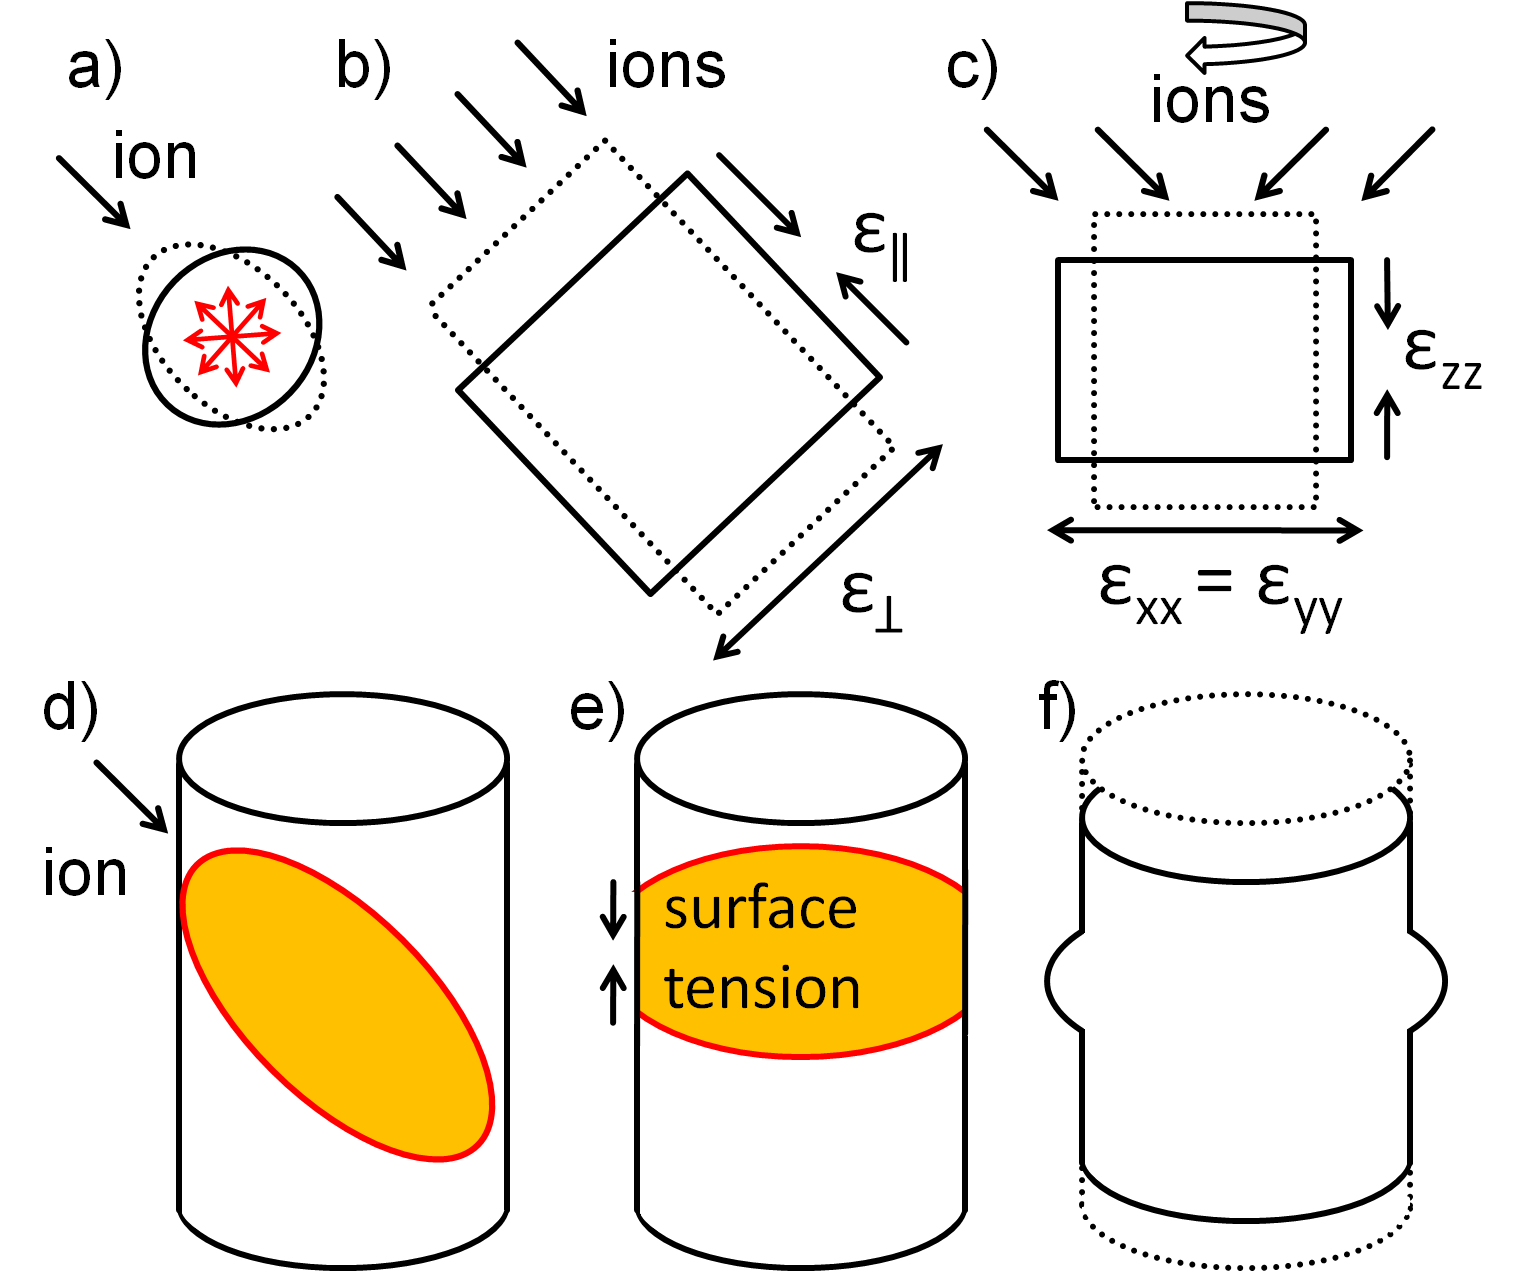
\includegraphics[width=8cm]{images/deformationmodel.jpg}
	\caption{a) - c) Illustration of a deformation model analogous to ion hammering. a) The collision cascade from a single impinging ion heats an approximately ellipsoidal volume of the target material. The internal pressure will lead to an expansion towards a more spherical shape which is retained upon cooling. b) The net effect of many ions is thus a contraction parallel to and an expansion perpendicular to the ion beam. For no change in density $\epsilon_\parallel = -2\epsilon_\perp$ has to hold. c) Under rotational symmetry this deformation translates to a contraction in the rotational axis $z$ and an expansion in the perpendicular $x-y$ plane with $\epsilon_{zz} = -2\epsilon_{xx} = -\epsilon_\perp$. In d) - f) the alternative, surface tension driven deformation is illustrated. The collision-heated volume of target material shown in d). A significant slice of the wire shown in e) thus has a reduced viscosity. The surface energy is reduced by an increase in the local diameter of the wire, leading to a shortened and thickened wire segment shown in f).} 
	\label{deformationmodel}
\end{figure}

\section{The deformation mechanism}

The effect of anisotropic deformation within the collision cascade induced by the irradiation of nanowires is shown in figure \ref{deformationmodel}a - c. An approximately ellipsoidal volume of the target material is heated by the collision cascade. It expands, becoming more spherical and the anisotropic deformation is retained after cooling. The superimposition of many collision cascades with a similar effect leads to a net contraction along the ion beam $\epsilon_{\parallel} < 0$ and an expansion perpendicular to it $\epsilon_{\perp} > 0$ as shown in \ref{deformationmodel}b. To maintain constant density $-2\cdot\epsilon_{\perp} =  \epsilon_{\parallel}$. The rotational average of this deformation around the $z$-axis, as illustrated in \ref{deformationmodel}c, works out to be a contraction along the $z$-axis $\epsilon_{zz} = \frac{1}{2} \epsilon_{\parallel}$ and a corresponding expansion in the $xy$-plane for an angle of $\pm\, 45^\circ$ between the ion beam and the $z$-axis. The $z$-axis represents the nanowire axis, while the $xy$-plane is parallel to the nanowire diameter. Thus the deformation rate of $\frac{d\epsilon_{zz}}{d\Phi} = 3\%$ strain per $10^{16}\,ions/cm^2$ extracted from a linear fit to the reduction of the nanowire height can be transformed into a strain rate parallel to the ion beam of $\frac{d\epsilon_{\parallel}}{d\Phi} = 6\%$ strain per $10^{16}\,ions/cm^2$. This is much less than the values reported for the studies at higher energies reported in literature. In ref. \cite{dillen_ion_2003} $10^{-16}\,cm^2/ion$ were reported for $300\,keV\,Xe$ in silica nanoparticles and ref. \cite{baumer_prediction_2014} even arrives at $10^{-15}\,cm^2/ion$ with MD calculations in bulk. There are unfortunately no studies published on straining bulk silicon at these low ion energies. The bending of thinned $Si$-wafers similar to \cite{volkert_stress_1991,massl_stress_2008} would be measurable with the a straining rate of $6\%$ strain per $10^{16}\,ions/cm^2$ in a layer of $\approx 300\,nm$.

The quantitative discrepancy between the deformation observed in the experiments presented here and published studies may be attributed to the lower ion energy and one may gain confidence in this model due to the qualitative similarity to the MD simulations by Baumer et al. \cite{baumer_prediction_2014} also showing deformation anisotropy at relatively low ion energies. However, a further, major concern is the fact that in the presented experiments the collision cascade is not in bulk, but in a nanostructure were there is not much material around and it is not distributed around the cascade isotropically. If the ellipsoidal volume intersects the nanowire surface, the pressure from the thermal expansion will vent outward removing the force needed to drive the deformation. An more favorable model illustrates that the strong influence of the surface expected in nanowires can also lead to the observed plastic deformation. In figure \ref{deformationmodel}d the relation between the nanowire and collision cascade is shown. As there is not much material around, the temperature in a sizable slice of the nanowire will remain elevated for some time \cite{borschel_ion-solid_2012,greaves_enhanced_2013,anders_sputtering_2015,johannes_ion_2015}. In addition the ion irradiation will further reduce the viscosity \cite{snoeks_stress_1997,hu_burrowing_2002,mayr_mechanisms_2003}, allowing the surface tension to deform the nanowire by increasing the radius locally. The local increase in diameter reduces the total surface area and thus the surface energy. The wire subsequently becomes shorter and wider as shown in figure \ref{deformationmodel}f. 

Apart from the bulk deformation experiment already suggested, a further experiment which could distinguish which of the two models applies is the irradiation of the nanowires at $90^\circ$ between the nanowire axis and the ion beam. In this case if the first model similar to ion hammering applies the irradiation should produce slowly elongating wires with a reduced radius, as the positive $\epsilon_{\perp}$ is now parallel to the nanowire axis. On the other hand, if the surface tension driven model is applicable the nanowires will shrink regardless of the irradiation angle. Naturally, a similar nanowire-on-microwire setup to the one for irradiation at $135^\circ$ could be used to irradiate at $90^\circ$. It turns out however, that the irradiation at $90^\circ$ is extremely prone to bending the nanowires. Due to the bending, the angle between the nanowire and the ion beam varied during a rotation cycle so that a conclusive discrimination between the models can unfortunately not be made. The bending can be attributed to the $Pt$ deposited to glue the $Si$ nanowire onto the $Au$ microwire in the FIB. This deposition is concentrated at the base and on one side of the nanowire and thus suppresses the rotational symmetry of the deformation, leading to bending. In the irradiation at $135^\circ$ the base of the wire, where it is glued to the microwire, is shadowed from the ion beam by the microwire so that the nanowires are less likely to bend. 


\chapter{Summary and Outlook}





\TODO{check: Master Thesis Noack, Ogrisek, Conference proceding D. Sage, Rutherford, Nordlund}
\bibliography{DissBib}



\end{document}